% !TeX spellcheck = en_US
\chapter{General synthetic iterative scheme}
\label{chap:GSIS}

\index{general synthetic iterative scheme}

One of the central problems in the study of rarefied gas dynamics is to find the steady-state solution of the Boltzmann equation quickly. When the Knudsen number is large, i.e. the system is highly rarefied, the conventional iterative scheme introduced in section~\ref{steady_iteration} can lead to convergence within a few iterations. However, when the Knudsen number is small, i.e. the flow falls in the near-continuum regime, hundreds of thousands iterations are needed, and yet the ``converged'' solutions are prone to be contaminated by accumulated error and large numerical dissipation. In this chapter, we put forward a general synthetic iterative scheme (GSIS) to find the steady-state solutions of general rarefied gas flows within dozens of iterations at any Knudsen number. 

%The key ingredient of our scheme is that the macroscopic equations, which are solved together with the Boltzmann equation and help to adjust the VDF, not only asymptotically preserve the Navier-Stokes limit in the framework of Chapman-Enskog expansion, but also contain  Newton's law for stress and  Fourier's law for heat conduction explicitly. For this reason, the constraint that the spatial cell size should be smaller than the molecular mean free path is removed, and we do not need the complex evaluation of numerical flux at cell interfaces. What's more, as the GSIS does not rely on the specific kinetic model/collision operator, it can be naturally extended to quickly find converged solutions for mixture flows and even flows involving chemical reactions. 

%These two superior advantages are expected to accelerate the slow convergence in simulation of near-continuum flows via the direct simulation Monte Carlo method and its low-variance version. 


\section{Problems of CIS }
%2020SUSTech/papers/SIAM_UPGSIS/Latex20200703/GSIS3

\begin{figure}[t]
	\centering
	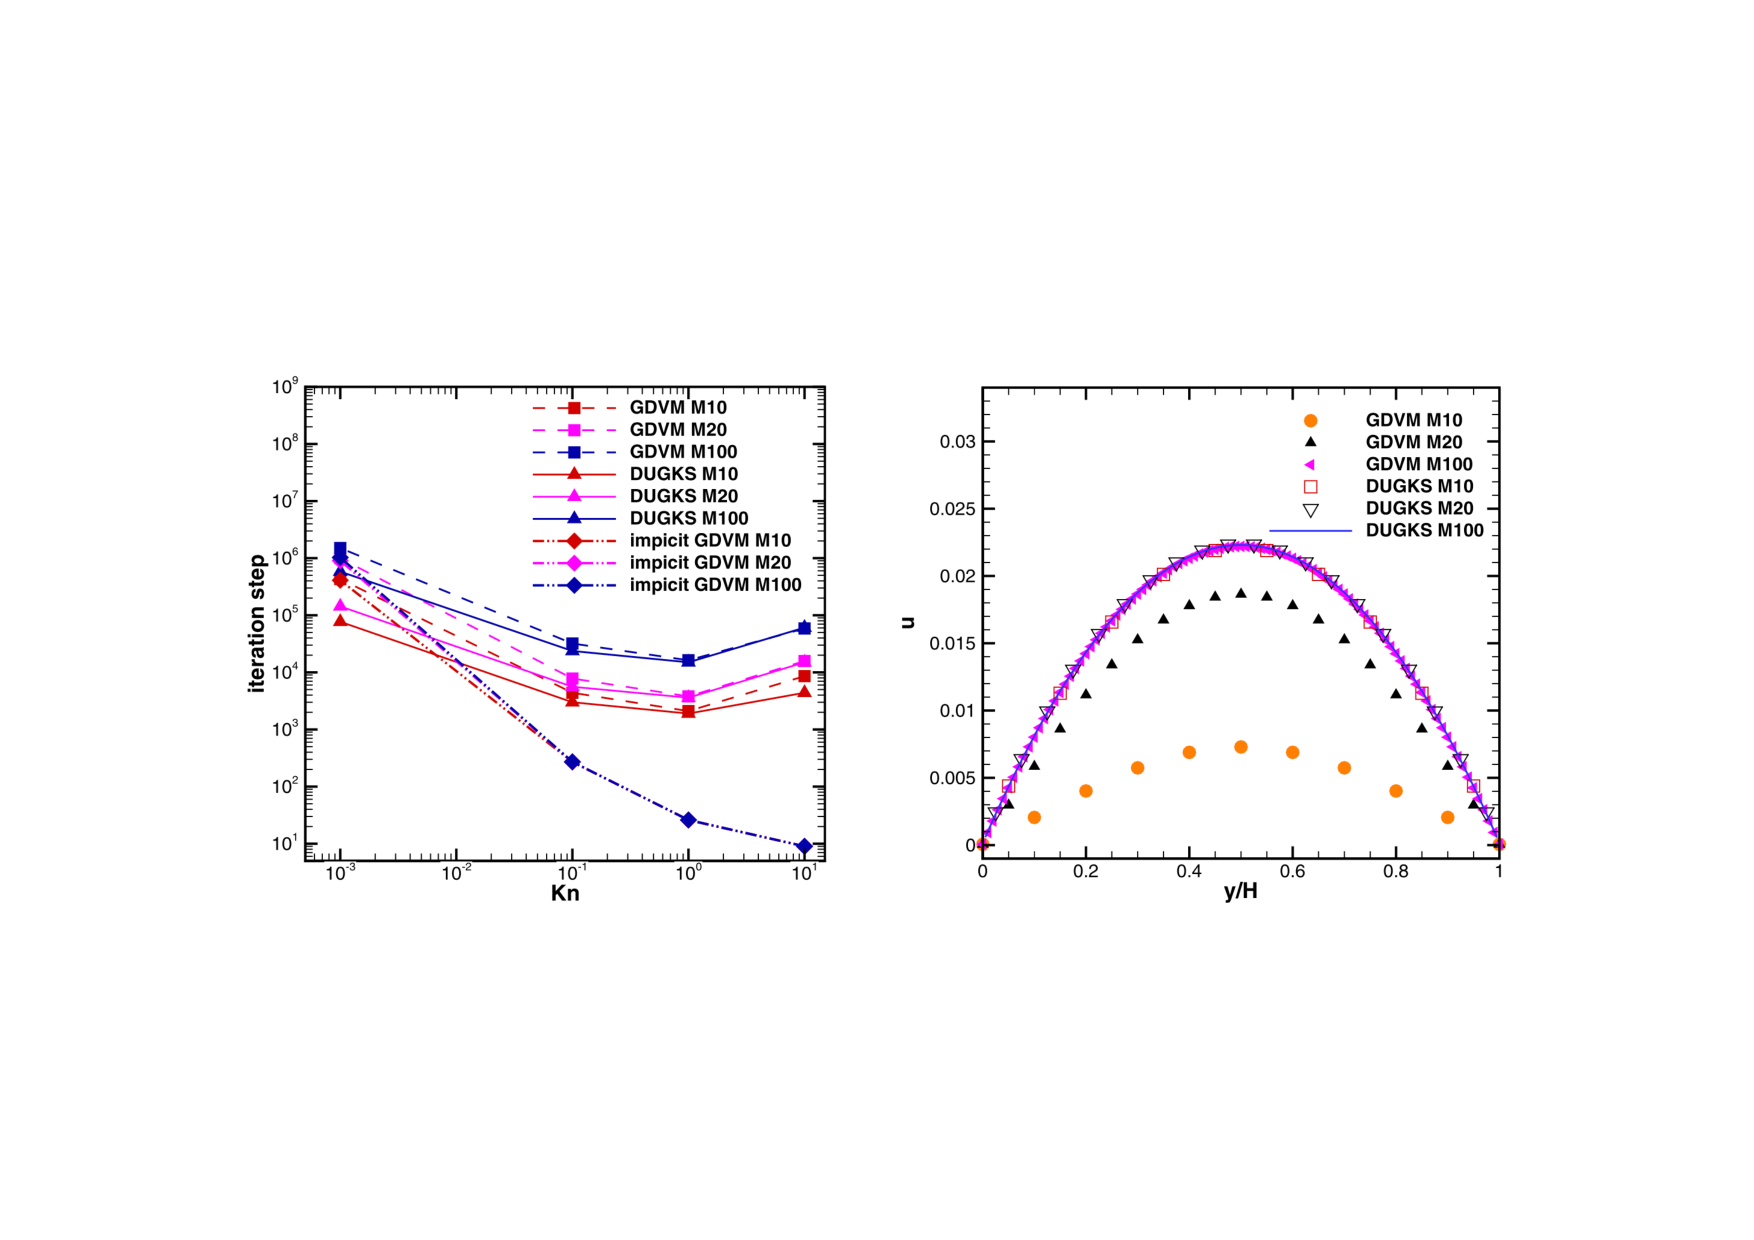
\includegraphics[scale=0.6]{Peng_CAF}
	\caption{ (Left) The iterative number needed to find the steady-state solution of force-driven Poiseuille flow, for the conventional iterative scheme and the DUGKS. M in the legend stands for the number of spatial cells. (Right) Velocity profiles obtained at different numbers of spatial cells when  $\text{Kn}=0.001$, which demonstrated that the CIS is highly dissipative~\cite{WANG201833}.  }
	\label{fig:Peng_CAF}
\end{figure}


To make the mathematical derivation simple but keep the essential flow physics, we consider the linearized BGK equation in general two-dimensional problems:
\begin{equation}\label{LBE_BGK}
\bm{v}\cdot\frac{\partial{h}(\bm{x},\bm{v})}{\partial\bm{x}}=\frac{h_{eq}(\bm{x},\bm{v})-h(\bm{x},\bm{v})}{K},
\end{equation}
where $h(\bm{x},\bm{v})$ is the VDF at location $\bm{x}=(x_1,x_2)$, $\bm{v}=(v_1,v_2)\in \mathbb{R}^2$ is the molecular velocity, $K$ is the inverse rarefaction parameter (here we will call it the Knudsen number), and $h_{eq}$ is the reference velocity distribution function:
\begin{equation}\label{LBE_BGK_gain}
h_{eq}(\bm{x},\bm{v})=\varrho(\bm{x})+2\bm{u}(\bm{x})\cdot\bm{v}+\tau(\bm{x})\left(v^2-1\right),
\end{equation}
with $\varrho$, $\bm{u}=(u_1,u_2)$ and $\tau$ being the density, flow velocity and temperature deviated from the global equilibrium state, respectively. They are related to the velocity distribution function $h$ as 
\begin{eqnarray}\label{Macro0}
M(\bm{x})=[\varrho,u_1,u_2,\tau]=\int{m}{h(\bm{x},\bm{v})}E(\bm{v}) d\bm{v},
\end{eqnarray}
where ${E}(\bm{v})=\exp(-v^2)/\pi$ is the velocity distribution function at global equilibrium and $m=[1,v_1, v_2, v^2-1]$ are the collisional invariants. Also, the shear stress $\sigma_{ij}$ (with $i,j=1,2$) and heat flux $q_i$ are defined as
\begin{eqnarray}
\sigma_{ij}(\bm{x})=2\int \left(v_iv_j-\frac{v^2}{2}\delta_{ij}\right)h(\bm{x},\bm{v})E(\bm{v})d\bm{v}, \label{NS_shear_def}\\
q_i(\bm{x})=\int {v_i}\left(v^2-2\right)h(\bm{x},\bm{v})E(\bm{v})d\bm{v}. \label{NS_heat_def}
\end{eqnarray}

%Note that the spatial variable $\bm{x}$ and molecular velocity $\bm{v}$ have been normalized by the mean free path and the most probable speed of gas molecules, respectively. %Also, the Prandtl number from the Chapman-Enskog expansion of Eq.~\eqref{LBE_BGK} is $\text{Pr}=1$.



%\section{Spectral radius of convergence}  %  tractable

%In this section we introduce both the CIS and GSIS, which are used to find the steady-state solution of the kinetic equation~\eqref{LBE_BGK}. Although in practical calculation the derivative with respect to $\textbf{x}$ can be approximated by  conventional CFD schemes such as the finite difference, finite volume, or Discontinuous Galerkin (DG) methods~\cite{WeiSuJCP1,Su2019IDG}, in the calculation of spectral radius of convergence, the spatial derivative is not discretized in order to keep the calculation tractable.


In CIS, given the value of VDF $h^{(k)}(\bm{x},\bm{v})$ at the $k$-th iteration step, its value at the next iteration step is calculated by solving the following equation:
\begin{equation}\label{LBE_iteration}
h^{(k+1)}+
K\bm{v}\cdot\frac{\partial
	{h}^{(k+1)}}{\partial{\bm{x}}}=h_{eq}(h^{(k)}),
\end{equation}
and the process is repeated until the maximum relative difference between successive estimates of macroscopic quantities, e.g. 
\begin{equation}\label{general_epsilon}
\epsilon=max\left\{\sqrt{\frac{\int|M^{(k+1)}-M^{(k)}|^2\mathrm{d}\bm{x}}{\int|M^{(k+1)}|^2\mathrm{d}\bm{x}}}\right\},
\end{equation}
is less than a preassigned value.

Although in practical numerical simulations the streaming operator $\partial/\partial{\bm{x}}$ is discretized, e.g. by the finite-difference, finite-volume, or discontinuous Galerkin (DG) methods~\cite{WeiSuJCP1,Su2019IDG}, here it is kept intact when calculating the convergence rate of iteration; that of the discretized version of Eq.~\eqref{LBE_iteration} will be tested in numerical simulations below.  

To calculate the convergence rate, we first define the following error function between the velocity distribution functions at two consecutive iteration steps:
\begin{eqnarray}
Y^{(k+1)}(\bm{x},\bm{v})=h^{(k+1)}(\bm{x},\bm{v})-h^{(k)}(\bm{x},\bm{v}), \label{Y_expression}
\end{eqnarray}
where according to Eq.~\eqref{LBE_iteration} the error function $Y^{(k+1)}(\bm{x},\bm{v})$ is found to satisfy
\begin{equation}\label{LBE_iteration2}
Y^{(k+1)}+
K\bm{v}\cdot\frac{\partial
	{Y}^{(k+1)}}{\partial{\bm{x}}}=\Phi_\varrho^{(k)}+2\Phi_{u_1}^{(k)}v_1+2\Phi_{u_2}^{(k)}v_2+\Phi_\tau^{(k)}\left(v^2-1\right),
\end{equation}
with the following error functions for the macroscopic quantities between two consecutive iteration steps: 
\begin{eqnarray}
\Phi^{(k+1)}_M(\bm{x})=M^{(k+1)}(\bm{x})-M^{(k)}(\bm{x})={\int{}mY^{(k+1)}(\bm{x},\bm{v})E(\bm{v})d\bm{v}}. \label{Phi_expression}
\end{eqnarray}


Second, to determine the convergence rate ${g}$ we perform the Fourier stability analysis by seeking the eigenvalue ${g}$ and eigenfunctions $y(\bm{v})$ and $\alpha_M=[\alpha_\varrho,\alpha_{u_1}, \alpha_{u_2}, \alpha_\tau]$  of the following forms:
\begin{eqnarray}
Y^{(k+1)}(\bm{x},\bm{v})={g}^{k}y(\bm{v})\exp(i\bm{\theta}\cdot{\bm{x}}),\label{Y_ansatz} \\
\Phi^{(k+1)}_{M}(\bm{x})={g}^{k+1}\alpha_M\exp(i\bm{\theta}\cdot{\bm{x}}), \label{Phi_ansatz}
\end{eqnarray}
where  $\bm{\theta}=(\theta_1,\theta_2)$ is the wave vector of perturbance. It should be noted that the factor ${g}^k$ emerges in Eq.~\eqref{Y_ansatz} rather than the factor ${g}^{k+1}$ in Eq.~\eqref{Phi_ansatz} because from Eq.~\eqref{LBE_iteration2} we know $Y^{(k+1)}$ is
determined by macroscopic quantities in the $k$-th iteration step. Obviously, when ${g}$ is very close zero, the iteration converges quickly. When ${g}$ is very close to one, the error between two consecutive steps rarely decreases, so the iteration converges extremely slowly. When $|{g}|>1$, the iteration will be unstable. 


Substituting Eqs.~\eqref{Y_ansatz} and~\eqref{Phi_ansatz} into Eqs.~\eqref{LBE_iteration2} and~\eqref{Phi_expression} we obtain the following expression for $y(\bm{v})$:
\begin{equation}\label{y_solution_CIS}
y(\bm{v})=\frac{\alpha_\varrho+2\alpha_{u_1}v_1+2\alpha_{u_2}v_2+\alpha_\tau(v^2-1)}{ 1+iK\bm{\theta}\cdot\bm{v} }.
\end{equation}
In the following we assume the wave vector of perturbation satisfies $|\bm{\theta}|^2=\theta_1^2+\theta_2^2=1$. Although in reality the perturbation may have various values of $\bm{\theta}$, their corresponding convergence rates do not interact because the kinetic equation is linear. Moreover, from the denominator in Eq.~\eqref{y_solution_CIS} we see that the convergence rate depends only on the product of $K\bm{\theta}$. If $|\bm{\theta}|\neq1$, the convergence rate at specific values of $\bm{\theta}$ and $K$ can be calculated by replacing the Knudsen number with $K|\bm{\theta}|$. 


Finally, with Eqs.~\eqref{Phi_expression}, \eqref{Y_ansatz}, \eqref{Phi_ansatz} and~\eqref{y_solution_CIS}, we obtain four linear algebraic equations for unknowns $\alpha_M$ that can be written in the matrix form as
\begin{equation}
C\alpha_M^\top={g}\alpha_M^\top,
\end{equation} 
where the superscript $\top$ is the transpose operator, and the $4\times4$ matrix $C$ reads
\begin{equation}\label{CIS}
C=\left[ \begin {array}{cccccc} 
\int{y_0d\bm{v}} & 2\int{v_1y_0d\bm{v}}& 2\int{v_2y_0d\bm{v}} & \int{Vy_0d\bm{v}} 
\\ \noalign{\medskip}
\int{v_1y_0d\bm{v}} & 2\int{v_1^2y_0d\bm{v}}& 2\int{v_1v_2y_0d\bm{v}} & \int{v_1Vy_0d\bm{v}}
\\ \noalign{\medskip}
\int{v_2y_0d\bm{v}} & 2\int{v_1v_2y_0d\bm{v}}& 2\int{v_2^2y_0d\bm{v}} & \int{v_2Vy_0d\bm{v}}
\\ \noalign{\medskip}
\int{Vy_0d\bm{v}} & 2\int{Vv_1y_0d\bm{v}}& 2\int{Vv_2y_0d\bm{v}} & \int{V^2y_0d\bm{v}} 
\end {array} \right], 
\end{equation}
with $V=v^2-1$ and
\begin{equation}\label{key_y0}
y_0(\bm{v})=\frac{E(\bm{v})}{1+iK\bm{\theta}\cdot\bm{v}}.
\end{equation}


In general, the value of ${g}$ can be obtained by numerically computing the eigenvalues ${g}$ of matrix $C$. The magnitude of the largest eigenvalue, i.e. the spectral radius, is the convergence rate. The result of spectral radius as a function of the Knudsen number is shown in Figure~\ref{fig:SR}. Specifically, when $K\rightarrow0$, the eigenvalue can be calculated analytically. For simplicity, we take $\theta_1=1$ and $\theta_2=0$; since the problem is isotropic, any other combinations of $\theta_1$ and $\theta_2$ with the condition $\theta_1^2+\theta_2^2=1$ will lead to the same value of maximum absolute eigenvalue. In this case, Eq.~\eqref{key_y0} is approximated as
\begin{equation}
y_0(\bm{v})=(1-iKv_1-K^2v_1^2)E(\bm{v})+O(K^3),
\end{equation}
and the matrix $C$ is approximated as
\begin{equation}\label{CIS_taylor}
C=\left[ \begin {array}{cccccc} 
1-\frac{K^2}{2} & -iK & 0 & -\frac{K^2}{2}
\\ \noalign{\medskip}
-\frac{iK}{2} & 1-\frac{3K^2}{2}& 0 & -\frac{iK}{2}
\\ \noalign{\medskip}
0 & 0 & 1-\frac{K^2}{2} & 0
\\ \noalign{\medskip}
-\frac{K^2}{2} & -iK & 0 & 1-\frac{3K^2}{2}
\end {array} \right].
\end{equation}

The four eigenvalues of the matrix are ${g}_{1,2}=1-K^2/2$ and ${g}_{3,4}=1-3K^2/2\pm{}iK$. Therefore, the maximum absolute eigenvalue is 
\begin{equation}\label{analytical_CIS}
{g}_{CIS}=1-\frac{K^2}{2}.
\end{equation}



\begin{figure}[t]
	\centering
	\includegraphics[viewport=80 97 790 380, clip,scale=0.5]{SR_mod_2.eps}
	\caption{ (a) The spectral radius ${g}$ as a function of the Knudsen number $K$ in both CIS and GSIS. Note that $K_{th}$ is a threshold Knudsen number, which is used to define the correction coefficient $\beta$, see Eqs.~\eqref{GSIS_K3} and~\eqref{GSIS_K30}. (b) The maximum spectral radius ${g}$ in the whole range of Knudsen number as a function of $K_{th}$.  }
	\label{fig:SR}
\end{figure}


The fact that ${g}_{CIS}$ approaches one when $K\rightarrow0$ means that errors defined in Eqs.~\eqref{Y_expression} and~\eqref{Phi_expression} decay rather slowly. Worse still, the CIS encounters the problem of ``false convergence''. According to the analysis of Adam and Larsen for radiation transfer equation~\cite{DSA2002} (similar for the BGK equation here), if the iteration is terminated at the $(k+1)$-th step with the following convergence criterion
\begin{equation}\label{false_convergence}
|\Phi_M^{(k+1)}-\Phi_M^{(k)}|<\epsilon,
\end{equation}
then the relative difference from the true steady-state solution $\Phi_M$ of Eq.~\eqref{LBE_BGK} is estimated as
\begin{equation}\label{false_convergence2}
|\Phi_M^{(k+1)}-\Phi_M|<\frac{{g}_{CIS}}{1-{g}_{CIS}}\epsilon\rightarrow\frac{2\epsilon}{K^2}, \quad \text{when~}K\rightarrow0.
\end{equation}
The asymptotic expression~\eqref{analytical_CIS} at $K\rightarrow0$ shows that, if the convergence criterion is chosen as Eq.~\eqref{false_convergence}, the error in the final iteration can be much larger than the preassigned value $\epsilon$; thus false convergence occurs if $\epsilon$ is not small enough. To reach the same convergence criterion for $|\Phi_M^{(k+1)}-\Phi_M|$, the total number of iterations must scale as $O(K^{-N})$ with $N>2$. This proves that in CIS it is very hard to obtain the converged solution in the near-continuum flow regime, see Figure~\ref{fig:Peng_CAF} for an example.




\section{Synthetic iterative scheme}


In recent years, the synthetic iterative scheme (SIS), which is initially developed for radiation transport processes~\cite{DSA2002}, has been extended to achieve high efficiency and accuracy in DVM, in particular with fast convergence property across the whole gas flow regimes~\cite{Valougeorgis:2003zr,Lihnaropoulos2007}. In this scheme, the gas kinetic equation and macroscopic equations are solved simultaneously on the same grids in the entire domain. Since the velocity distribution function is guided by the macroscopic flow quantities solved from diffusion-type equations at each iterative step, information propagates accurately and fast even when Knudsen number is small. When the Knudsen number is small, the synthetic macroscopic equations asymptotically approach the Navier-Stokes equations. On the other hand, the SIS also preserves accuracy in other flow regimes since the macroscopic equations contains high-order terms to take into account rarefaction effects. The SIS has been successfully applied to Poiseuille flow in channels of arbitrary shapes using the BGK kinetic model for single-species monatomic gases~\cite{SZALMAS20104315}, and flows of binary and ternary gas mixtures driven by local pressure, temperature and concentration gradients using the McCormak model~\cite{NARIS2004629,NARIS2004294,Naris2005Pof,SZALMAS201691}. It has also been extended to solve the linearized Boltzmann equation (LBE), where the role of realistic intermolecular potentials in Poiseuille, Couette and thermal transpiration flows has been analyzed~\cite{LeiJCP2017,SU2019573}.


It is interesting to note that the similar idea of SIS has also been used in DSMC, that is, in addition to traditional DSMC, macroscopic variables are solved and updated according to macroscopic rules/equations. For instances, in the information preservation DSMC, the information velocity is introduced to compute macroscopic velocity and shear stress, with the aim of removing ``the statistical fluctuation source inherent in the DSMC method that results from the randomness of the thermal velocity''~\cite{Fan2001,ZhangJun2011JCP,Fei2013}, although the rule of updating the information velocity and/or other macroscopic variables is not exactly derived from the Boltzmann equation. On the other hand, the moment-guided DSMC is proposed to reduce the statistical error, where the density, velocity and temperature are updated by the five exact macroscopic equations from conservation laws, but with the pressure tensor and heat flux calculated from the DSMC~\cite{Degond2011}. Similar idea is adopted in neutral gas kinetics, where, in addition to the five macroscopic equations for density, velocity and temperature, consistency terms are introduced to ensure that, upon convergence, solutions from the low-order macroscopic equations will be the same as that from the kinetic equations~\cite{Taitano2014}. Although fast convergence is realized, this, however, will cause problems since if the spatial cell size is not resolved the DVM solution of gas kinetic equations is contaminated by the large numerical dissipation, for instances. 


In DVM, the SIS can not only asymptotically achieve the Navier-Stokes limit with fast convergence rate, but also preserve accuracy in high Knudsen number regimes. The critical point to develop this scheme is that the macroscopic equations must explicitly contain both the constitutive relations predicting the transport phenomena at the continuum level, and high-order terms taking into accounting rarefaction effects. To the author's awareness, in rarefied gas dynamics the SIS is still limited to simple flows such as the Poiseuille, Couette and thermal transpiration flows, where the flow velocity is perpendicular to the computational domain, we refer to~\cite{Valougeorgis:2003zr} for an example.




\section{General synthetic iterative scheme}\label{secIII}

In this section we develop the general synthetic iterative scheme to handle the general rarefied gas flows. For simplicity we first consider the 2D linearized BGK equation~\eqref{LBE_BGK}. 

\subsection{Fast convergence}

In GSIS, additional macroscopic equations are coupled with CIS to boost convergence~\cite{SuArXiv2019}. The algorithm is summarized below. First, given the value of velocity distribution function $h^{(k)}(\bm{x},\bm{v})$ at the $k$-th iteration step, the velocity distribution function at the intermediate $(k+1/2)$-th step is obtained by solving the following kinetic equation: 
\begin{equation}\label{LBE_iteration_2}
h^{(k+1/2)}+
K\bm{v}\cdot\frac{\partial
	{h}^{(k+1/2)}}{\partial{\bm{x}}}=h_{eq}(h^{(k)}).
\end{equation}


Second, macroscopic quantities $\bar{M}=(\bar{\varrho},\bar{u}_1,\bar{u}_2, \bar{\tau})$ are introduced to update $M$ at the (k+1)-th iteration step in the following manner:
\begin{equation}\label{GSIS_K30}
M^{(k+1)}=\beta\bar{M}+(1-\beta)M^{(k+1/2)},
\end{equation} 
where $0\le\beta\le1$ is the relaxation coefficient: when $\beta=0$ the scheme is reduced to the CIS with no fast convergence at small Knudsen numbers. The macroscopic quantities $\bar{M}$ at the $(k+1)$-th iteration step can be obtained by solving the following partial differential equations (note that the Einstein summation is used):
\begin{eqnarray}
\frac{\partial {\bar{u}_i}}{\partial{x_i}}=0, \label{macro_1} \\
\frac{\partial {\bar{\varrho}}}{\partial{x_i}}+\frac{\partial {\bar{\tau}}}{\partial{x_i}}+\frac{\partial {\bar{\sigma}_{ij}}}{\partial{x_j}}=0, \label{macro_2} \\
\frac{\partial {\bar{q}_i}}{\partial{x_i}}=0, \label{macro_3}
\end{eqnarray}
which are obtained by taking the velocity moments of the BGK equation~\eqref{LBE_BGK}. However, in GSIS the shear stress $\bar{\sigma}_{ij}$ and heat flux $\bar{q}_i$ are not directly calculated from the velocity distribution function $h^{(k+1/2)}$ according to Eqs.~\eqref{NS_shear_def} and~\eqref{NS_heat_def}, but are reconstructed as
\begin{eqnarray}
\bar{\sigma}_{ij} =-2K_e\frac{\partial \bar{u}_{<i}}{\partial {x_{j>}}}+\text{HoT}_{\sigma_{ij}}, \label{sigma_BGK_HoT}\\
\bar{q}_i =-K_e\frac{\partial \bar{\tau}}{\partial x_i}+\text{HoT}_{q_i}, \label{q_BGK_HoT}
\end{eqnarray} 
such that Eqs.~\eqref{macro_1}, \eqref{macro_2} and~\eqref{macro_3} are reduced to the linearized Navier-Stokes equations when the high-order terms $\text{HoT}_{\sigma_{ij}}$ and $\text{HoT}_{q_i}$ vanish, and when $K_e$ takes the value of $K$; the role of $K_e$ will be discussed below in section~\ref{sec:whyimportant}, where we will show the inclusion of Newton's law for shear stress and Fourier's law for heat conduction in Eqs.~\eqref{sigma_BGK_HoT} and~\eqref{q_BGK_HoT} is critical to realize the fast convergence in the near-continuum flow regime. Note that the high-order terms $\text{HoT}_{\sigma_{ij}}$ and $\text{HoT}_{q_i}$ should be derived exactly from the kinetic equation~\eqref{LBE_BGK}, so that the rarefaction effects beyond the Navier-Stokes level are all captured. 


There are many ways to construct the expressions for these high-order terms. In our  paper~\cite{SuArXiv2019}, they are constructed by multiplying Eq.~\eqref{LBE_BGK} with $\left(v_iv_j-{v^2}\delta_{ij}/2\right)E$ and ${v_i}\left(v^2-2\right)E$, respectively, and integrating the resultant equations with respect to the molecular velocity $\bm{v}$: 
\begin{eqnarray}
\text{HoT}_{\sigma_{ij}}=2K_e\frac{\partial u^{(k+1/2)}_{<i}}{\partial {x_{j>}}}-2K\int{\left(v_iv_j-\frac{v^2}{2}\delta_{ij}\right)}\bm{v}\cdot\frac{\partial{} h^{(k+1/2)}}{\partial\bm{x}}d\bm{v}, \label{higher_order_app1}\\
\text{HoT}_{q_i} =K_e\frac{\partial \tau^{(k+1/2)}}{\partial x_i}-K\int{v_i(v^2-2)}\bm{v}\cdot\frac{\partial{} h^{(k+1/2)}}{\partial\bm{x}}d\bm{v}. \label{higher_order_app2}
\end{eqnarray}



Clearly, the above high-order terms are correct when the steady state is reached. However, during iteration when the steady state is not reached, Eqs.~\eqref{sigma_BGK_HoT} and~\eqref{q_BGK_HoT} are not correct since macroscopic quantities $\bar{M}$ are evaluated at the $(k+1)$-th iteration step, while high-order terms $\text{HoT}_{\sigma_{ij}}$ and $\text{HoT}_{q_i}$ are computed using the intermediate velocity distribution function at the $(k+1/2)$-th iteration step. %Theoretically they can be both evaluated at the  $(k+1)$-th iteration step, but the calculation of differential-integral equation is extremely time consuming.




\subsubsection{The case of $\beta=1$ and $K_e=K$} To calculate the convergence rate of GSIS, we introduce the error function for the velocity distribution function as
\begin{eqnarray}
Y^{(k+1/2)}(\bm{x},\bm{v})=h^{(k+1/2)}(\bm{x},\bm{v})-h^{(k)}(\bm{x},\bm{v})={g}^{k}y(\bm{v})\exp(i\bm{\theta}\cdot{\bm{x}}),\label{Y_ansatz2} 
\end{eqnarray}
while the error functions $\Phi_M$ are still defined as $\Phi^{(k+1)}_M(\bm{x})=M^{(k+1)}(\bm{x})-M^{(k)}(\bm{x})$. It is clear that, according to Eq.~\eqref{LBE_iteration_2}, the solution of $y(\bm{v})$ is still given by Eq.~\eqref{y_solution_CIS}. It should be emphasized that, in GSIS the error functions $\Phi_M$ are not directly calculated from $Y$, but are calculated from macroscopic synthetic equations; the equations for $\Phi^{(k+1)}_M(\bm{x})$ are given by Eqs.~\eqref{macro_1}-\eqref{higher_order_app2}, if $\bar{\varrho},\bar{u}_1,\bar{u}_2$ and $\bar{\tau}$ are replaced by $\Phi_\rho^{(k+1)}$, $\Phi_{u_1}^{(k+1)}$, $\Phi_{u_2}^{(k+1)}$ and $\Phi_\tau^{(k+1)}$, respectively, and $h(\bm{x},\bm{v})$ is replaced by $Y(\bm{x},\bm{v})$.  

%Instead, macroscopic quantities $M^{(k+1)}(\bm{x})$  are governed by Eqs.~\eqref{macro_1}, \eqref{macro_2} and~\eqref{macro_3}, from which one can obtain the governing equations for $\Phi^{(k+1)}_M(\bm{x})$. \lei{To be specific, }


On substituting Eqs.~\eqref{Y_ansatz2}, \eqref{Phi_expression} and  \eqref{Phi_ansatz} into the governing equations for $\Phi^{(k+1)}_M(\bm{x})$, we obtain the following four linear algebraic equations:
\begin{eqnarray}
{g}(i\theta_1\alpha_{u_1}+i\theta_2\alpha_{u_2})=0, \label{GSIS_first}\\
{g}[i\theta_1(\alpha_\varrho+\alpha_\tau)+K_e\alpha_{u_1}]=S_1,\\
{g}[i\theta_2(\alpha_\varrho+\alpha_\tau)+K_e\alpha_{u_2}]=S_2,\\
{g}{K_e}\alpha_{\tau}=S_\tau, \label{GSIS_middle1}
\end{eqnarray}
where the source terms, due to high-order terms in Eqs.~\eqref{higher_order_app1} and~\eqref{higher_order_app2}, are also linear functions of $\alpha_M$: $S_1=\int{s_1}yEd\bm{v}$, $S_2=\int{s_2}yEd\bm{v}$, and $S_\tau=\int{s_\tau}yEd\bm{v}$, with
\begin{eqnarray}
s_1=K_ev_1+K(i\theta_1v_1+i\theta_2v_2)\left[i\theta_1(v_1^2-v_2^2)+2i\theta_2v_1v_2\right], \label{GSIS_middle2}\\
s_2=K_ev_2+K(i\theta_1v_1+i\theta_2v_2)\left[2i\theta_1v_1v_2+i\theta_2(v_2^2-v_1^2)\right], \\
s_\tau=K_e(v^2-1)+K(i\theta_1v_1+i\theta_2v_2)\left(i\theta_1v_1+i\theta_2v_2\right)(v^2-2). \label{GSIS_end}
\end{eqnarray} 



The spectral radius of GSIS can be obtained by solving Eqs.~\eqref{GSIS_first}-\eqref{GSIS_end}. That is, these equations are firstly rewritten in the matrix form as
\begin{equation}
L{g}\alpha_M^\top=R\alpha_M^\top,
\end{equation} 
where the $4\times4$ matrix $L$ is obtained from the left-hand side of equations~\eqref{GSIS_first}-\eqref{GSIS_middle1} as:
\begin{equation}\label{GSIS_L}
L=\left[ \begin {array}{cccccc} 
0& i\theta_1& i\theta_2 &0 
\\ \noalign{\medskip}
i\theta_1 &K_e &0 &i\theta_1 
\\ \noalign{\medskip}
i\theta_2 &0 &K_e &i\theta_2 
\\ \noalign{\medskip}
0  &0  & 0 &K_e
\end {array} \right], 
\end{equation}
and due to the fact that $y(\bm{v})$ in Eq.~\eqref{y_solution_CIS} a linear combination of $\alpha_\varrho, \alpha_{u_1}, \alpha_{u_2}$ and $\alpha_{\tau}$, the $4\times4$ matrix $R$ is obtained from Eqs.~\eqref{GSIS_middle2}-\eqref{GSIS_end} as 
\begin{equation}\label{GSIS_R}
R=\left[ \begin {array}{cccccc} 
0& 0 & 0 & 0 
\\ \noalign{\medskip}
\int{y_0s_1d\bm{v}} & 2\int{v_1y_0s_1d\bm{v}}& 2\int{v_2y_0s_1d\bm{v}} & \int{Vy_0s_1d\bm{v}}
\\ \noalign{\medskip}
\int{y_0s_2d\bm{v}} & 2\int{v_1y_0s_2d\bm{v}}& 2\int{v_2y_0s_2d\bm{v}} & \int{Vy_0s_2d\bm{v}}
\\ \noalign{\medskip}
\int{y_0s_\tau{}d\bm{v}} & 2\int{v_1y_0s_\tau{}d\bm{v}}& 2\int{v_2y_0s_\tau{}d\bm{v}} & \int{Vy_0s_\tau{}d\bm{v}}
\end {array} \right].
\end{equation}

By introducing 
\begin{equation}\label{gsis_Matrix_G}
G=L^{-1}R
\end{equation}
and numerically computing the eigenvalues of the matrix $G$ we obtain the spectral radius ${g}$ of GSIS. The results are shown in the dotted black line in Figure~\ref{fig:SR}. 
Specifically, the analytical solution for $g$ can be obtained when $K$ approaches zero. Again here we choose $\theta_1=1$ and $\theta_2=0$ because the problem is isotropic. Also, we choose $K_e=K$; later in section~\ref{sec:whyimportant} we will find that this leads to the smallest spectral radius when $K\rightarrow0$. Thus, we have
\begin{equation*}\label{GSIS_taylor_invL}
L^{-1}=\left[ \begin {array}{cccccc} 
K & -i & 0 & -\frac{1}{K}
\\ \noalign{\medskip}
-i & 0 & 0 & 0
\\ \noalign{\medskip}
0 & 0 & \frac{1}{K} & 0
\\ \noalign{\medskip}
0 & 0 & 0 & \frac{1}{K}
\end {array} \right], \quad \text{and~}
R=\left[ \begin {array}{cccccc} 
0 & 0 & 0 & 0
\\ \noalign{\medskip}
0 & \frac{3K^3}{2}& 0 & \frac{iK^2}{2}
\\ \noalign{\medskip}
0 & 0 & K^3 & 0
\\ \noalign{\medskip}
\frac{K^3}{4} & \frac{iK^2}{2} & 0 & \frac{9K^3}{4}
\end {array} \right].
\end{equation*}
Therefore, the matrix $G$ is expressed as
\begin{equation}\label{GSIS_taylor_G}
G=\left[ \begin {array}{cccccc} 
-\frac{K^2}{4} & -\frac{iK}{2} & 0 & -\frac{7K^2}{4}
\\ \noalign{\medskip}
0 & 0 & 0 & 0
\\ \noalign{\medskip}
0 & 0 & K^2 & 0
\\ \noalign{\medskip}
\frac{K^2}{4} & \frac{iK}{2} & 0 & \frac{9K^2}{4}
\end {array} \right],
\end{equation}	
where the four eigenvalues are $\omega_1=0$, $\omega_2=K^2$, and $\omega_{3,4}=K^2(1\pm3/2\sqrt{2})$. The maximum absolute eigenvalue is
\begin{equation}\label{analytical_gsis_max}
{g}=\left(1+\frac{3}{2\sqrt{2}}\right)K^2\approx2.06K^2.
\end{equation}
This demonstrates that the GSIS is able to boost convergence significantly in the near-continuum flow regime. However, the spectral radius increases to one when $K\rightarrow\infty$. This stands in sharp contrast to DSA schemes for rarefied Poiseuille-type flows, where the flow velocity (only in one direction) is perpendicular to spatial variables~\cite{Valougeorgis:2003zr}. As a consequence, the synthetic equation for the only flow velocity is of diffusion-type~\cite{Valougeorgis:2003zr,LeiJCP2017,SU2019573}, and the spectral radius goes to zero when $K\rightarrow\infty$ and $K\rightarrow0$. However, in GSIS we have multiple flow velocities whose directions are inside the spatial domain, and the synthetic equations contain the continuity equation~\eqref{macro_1} which is not of diffusion type. Comparing GSIS with DSA, the continuity equation  might be  the reason that the spectral radius goes to one at large Knudsen numbers. This problem is fixed below.


\subsubsection{The case of $\beta<1$ and $K_e=K$} To make the spectral radius in GSIS goes to zero at large Knudsen numbers, the relaxation coefficient in Eq.~\eqref{GSIS_K30} is chosen as
\begin{equation}\label{GSIS_K3}
\beta=\frac{min(K,K_{th})}{K},
\end{equation}
where $K_{th}$ is the threshold Knudsen number, so that GSIS is reduced to CIS when $K$ is much larger than $K_{th}$, where the spectral radius approaches zero. Mathematically, the spectral radius of this GSIS can be obtained by computing the eigenvalue of the matrix
\begin{equation}
G=\beta{L^{-1}R}+(1-\beta)C,
\end{equation} 
where the results at the threshold Knudsen number of values 1 and 4 are shown in Figure~\ref{fig:SR}(a). Clearly, by choosing approximate value of $\beta$ (or $K_{th}$), we can make the maximum value of ${g}$ less than 0.5; from Figure~\ref{fig:SR}(b) we see that the range for $K_{th}$ is board, i.e. it can vary from 0.5 to 4. This means that after 10 iterations, the error will be decreased by three orders of magnitude. Thus, theoretically, GSIS permits fast convergence in the whole range of Knudsen number, which has been demonstrated by the numerical examples in our recent paper~\cite{SuArXiv2019}.


In addition to the fast convergence at large Knudsen numbers, Eq.~\eqref{GSIS_K3} with $\beta<1$ can make the algorithm more stable. This is because, when $K$ is large, high-order terms defined in Eqs.~\eqref{higher_order_app1} and~\eqref{higher_order_app2} may have strong variations around sharp (i.e. rectangular) corners, which leads to unphysical variations of density, velocity and temperature when solving Eqs.~\eqref{macro_1}, \eqref{macro_2} and~\eqref{macro_3}. By updating the macroscopic quantities according to Eq.~\eqref{GSIS_K30}, the error at sharp boundaries is reduced and stable algorithm is guaranteed~\cite{SuArXiv2019}. 


\begin{figure}[t]
	\centering
	\includegraphics[scale=0.45]{whyimportant.eps}
	\caption{ The spectral radius ${g}$ as a function of the Knudsen number $K$ in GSIS, when $K_e$ in Eqs.~\eqref{sigma_BGK_HoT} and~\eqref{q_BGK_HoT} takes different values and the relaxation coefficient  in Eq.~\eqref{GSIS_K30} is $\beta=1$. }
	\label{fig:whyimportant}
\end{figure}




\subsection{Importance of NSF constitutive relations}\label{sec:whyimportant}

Note that when the Knudsen number is small, we choose $\beta=1$ in Eq.~\eqref{GSIS_K30} and $K_e=K$ in Eqs.~\eqref{sigma_BGK_HoT} and~\eqref{q_BGK_HoT}; this means that in the near-continuum regime, the constitutive relations in Navier-Stokes equations, i.e. Newton's law for shear stress and Fourier's law for heat conduction, are explicitly included in the macroscopic synthetic equations. This turns out to be extremely important for the fast convergence of GSIS, as the spectral radius goes to zero when $K\rightarrow0$, see Figure~\ref{fig:SR} and Eq.~\eqref{analytical_gsis_max}.


To demonstrate this superiority, we calculate the spectral radius ${g}$ by choosing different values of $K_e$ when the Knudsen number $K$ is small; the results in Figure~\ref{fig:whyimportant} show that only when $K_e=K$ can the spectral radius go to zero when $K\rightarrow0$. Moreover, when $K<0.2$, the further  $K_e$ deviates away from $K$, the larger the spectral radius and hence the slower the convergence. When $K_e$ deviates too much from $K$, say $K_e=0.45K$, ${g}$ can be even larger than one, which means that the GSIS is unstable. In the extreme case $K_e/K\rightarrow0$, from the numerical solutions we find that ${g}\rightarrow{K/K_e}$. These results confirm that the fastest convergence can be realized by including the Navier-Stokes constitutive relations explicitly in macroscopic synthetic equations. The secret to the fast convergence of GSIS is that Eqs.~\eqref{macro_1}, \eqref{macro_2} and~\eqref{macro_3} are exactly the linearized Navier-Stokes equations of the corresponding linearized kinetic equation when higher-order terms are neglected, which lead to diffusion equations for the flow velocity and temperature; these diffusion equations enable efficient flow information exchange across the whole computational domain. If the shear stress and heat flux in Eqs.~\eqref{macro_2} and~\eqref{macro_3} are directly computed from the $h^{(k+1/2)}$ according to Eqs.~\eqref{NS_shear_def} and~\eqref{NS_heat_def},  there are no diffusion equations for the velocity and temperature. 
%Moreover, there are only three effective equations which cannot determine the four macroscopic quantities in the collision operator of the BGK equation, and hence no fast convergence in the near-continuum flow regime.  %As a matter of fact, taking $K_e=0$, one cannot even find the inverse of the matrix L in Eq.~\eqref{GSIS_L}. 


%This example shows that the macroscopic synthetic equations 

\subsection{Asymptotic preserving}

Note that in GSIS the kinetic equation and macroscopic synthetic equations can be solved by different numerical methods with different order of accuracy. Now we consider the influence of spatial discretization in the gas kinetic solver on the accuracy of GSIS, based on the assumptions that (i) synthetic equations can be solved exactly and (ii) the spatial cell size $\Delta{x}$ is able to capture the physical solution of the Navier-Stokes equation. To this end, we consider whether the Navier-Stokes equations can be derived or not, through the Chapman-Enskog expansion~\cite{CE}, from the discretized gas kinetic equation with the following scaling:
\begin{equation}\label{scaling}
\Delta{x}\sim{K^{1/\alpha}}.
\end{equation}
Here $\alpha$ denotes the order of accuracy in the asymptotic preserving of Navier-Stokes equations. Clearly, the larger the value of $\alpha$, the better the numerical scheme, as we can use less number of spatial cells to achieve the same accuracy. It has been rigorously proven that the discrete unified gas kinetic scheme has $\alpha=2$, so that $\Delta{x}$ can be much larger than the mean free path to capture the hydrodynamics in bulk regions~\cite{Guo2019UP_arXiv}. If $\alpha=\infty$, the scheme will capture the hydrodynamical behavior of gas when $\Delta{x}$ is approximately the system size (no matter what the value of $K$ is), as long as this size is adequate to capture the flow physics, for example the dynamics of a sound wave whose wavelength is approximately the system size.


Since the spectral radius of GSIS approaches zero when $K\rightarrow0$, the converged solution can be found within a few number of iterations, and we have $h_{eq}^{(k+1)}=h_{eq}^{(k)}$ and $M^{(k+1)}=M^{(k)}$. Thus, when the iteration is converged, the kinetic equation~\eqref{LBE_iteration_2} in the discretized form can be written as
\begin{equation}\label{LBE_GSIS}
\bm{v}\cdot\frac{\partial{h}}{\partial\bm{x}}+O(\Delta{x}^n)\delta(h)=\frac{h_{eq}-h}{K},
\end{equation}
where  $n$ is the order of approximation for the spatial derivative $\partial {h}/\partial{x}$, and $\delta(h)$ is the $(n+1)$-th order derivative of $h$. For instance, if the second-order upwind finite difference scheme, we have $n=2$. If the third-order approximating polynomials are used in the DG method~\cite{WeiSuJCP1,Su2019IDG}, we have $n=4$. %Obviously, the larger the value of $n$, more accurate solution can be obtained on coarse mesh. 





%Since in GSIS the mass, velocity and temperature are obtained from solving Eqs.~\eqref{macro_1} to~\eqref{higher_order_app2}, we find that if we have $h_0=h_{eq}$, the macroscopic synthetic equations are reduced to the linearized Navier-Stokes equation exactly.


%\begin{figure}[t]
%	\centering
%	\includegraphics[scale=0.7]{multiscale_framework}
%	\caption{Multiscale framework}
%	\label{fig:multiscale_framework}
%\end{figure}


In the Chapman-Enskog expansion the velocity distribution function is approximated by the Taylor expansion
$h=h_0+Kh_1+\cdots$.
By subsisting this expansion into Eq.~\eqref{LBE_GSIS} and collecting terms with the order of $K^{-1}$, we have $h_0=f_{eq}$, when the following largest scaling is chosen
\begin{equation}\label{scaling2}
\Delta{x}\sim{K^{1/\infty}}=O(1).
\end{equation}
Under the scaling~\eqref{scaling2}, by collecting terms with the order $K^{0}$, we have
$h_1=-\bm{v}\cdot{\partial{h_{eq}}}/{\partial\bm{x}}-\delta(h_{eq})$. Note that at small values of $K$ we have $\beta=1$ in Eqs.~\eqref{GSIS_K3} and~\eqref{GSIS_K30}. 
Thus, according to Eqs.~\eqref{sigma_BGK_HoT}, \eqref{q_BGK_HoT}, \eqref{higher_order_app1} and~\eqref{higher_order_app2}, Newton's law for shear stress and Fourier's law for heat conduction are recovered in macroscopic synthetic equations with accuracy $O(K^2)$:
\begin{eqnarray}
\sigma_{ij} =-2K\frac{\partial u_{<i}}{\partial {x_{j>}}}+O(K^2), \quad
q_i =-K\frac{\partial \tau}{\partial x_i}+O(K^2).
\end{eqnarray} 


Thus, as long as the spatial resolution $\Delta{x}=O(1)$ is able to capture the physical solution of the Navier-Stokes equation, GSIS is able to recover the linearized Navier-Stokes equations when $K\rightarrow0$; in this sense the GSIS is better than the discrete unified gas kinetic scheme~\cite{Guo2019UP_arXiv} where $\Delta{x}=O(\sqrt{K})$. Therefore, the overall order of accuracy of GSIS depends only on the order to solve macroscopic synthetic equations, that is, $n$ in Eq.~\eqref{LBE_GSIS}. In reality, however, such a large spatial cell size $\Delta{x}=O(1)$ cannot be used in regions with Knudsen layers or shock structures, where the physical solutions require a spatial resolution of $O(K)$. Fortunately, these kinetic layers only take up a small fraction of the computational domain, say, in the vicinity of solid walls, which can be captured by implicit schemes with non-uniform spatial discretization. This will be tested in the following numerical examples.





\section{GSIS for linearized Boltzmann equation}

The steady state solution of the integro-differential system~\eqref{Chapter1_Boltzmann_lin} is usually solved by the CIS. Given the value of $h^{(k)}(\bm{x},\bm{v})$ at the $k$-th iteration step, the velocity distribution function at the next iteration step is calculated by solving the following equation~\cite{ohwada1989numerical,Lei2013}:
\begin{equation}\label{LBE_Boltzmann_iteration}
\nu_{eq}(\bm{v})h^{(k+1)}+
\bm{v}\cdot\frac{\partial
	{h}^{(k+1)}}{\partial{\bm{x}}}=L^+(h^{(k)},f_{eq}),
\end{equation}



To this end, we first multiply Eq.~\eqref{Chapter1_Boltzmann_lin} by 1, 2$\bm{v}$, and $v^2-\frac{3}{2}$, respectively, and integrate the resultant equations with respect to $\bm{v}$; we obtain the following equations for the evolution of the density, velocity, and temperature: 
\begin{equation}\label{eq123}
\begin{aligned}
\frac{\partial {\rho}}{\partial{t}}+\frac{\partial {U_i}}{\partial{x_i}}=0, \\
2\frac{\partial {U_i}}{\partial{t}}+\frac{\partial {\rho}}{\partial{x_i}}+\frac{\partial {T}}{\partial{x_i}}+\frac{\partial {{\sigma_{ij}}}}{\partial{x_j}}=0, \\
\frac{3}{2}\frac{\partial {T}}{\partial{t}}+\frac{\partial {{q_j}}}{\partial{x_j}}+\frac{\partial {U_j}}{\partial{x_j}}=0,
\end{aligned}
\end{equation}
which are not closed, since expressions for the shear stress $\sigma_{ij}$ and heat flux $\bm{q}$ are not known. One way to close Eq.~\eqref{eq123} is to use the Chapman-Enskog expansion, where the distribution function is expressed in the power series of $\mathrm{Kn}$~\citep{CE}: $h=\mathrm{Kn} h^{(1)}+\mathrm{Kn}^2 h^{(2)}+\cdots$. When $f=f^{(0)}$, we have $\sigma_{ij}= q_i=0$, and Euler equations are recovered. When the distribution function is truncated at the first-order of $\mathrm{Kn}$, that is, $
h=\mathrm{Kn} h^{(1)}$,
we have 
\begin{equation}\label{GTMNSF}
\begin{aligned}[b]
\sigma_{ij} =-\delta_{rp}^{-1}\left(\frac{\partial U_{i}}{\partial x_{j}}+\frac{\partial U_{j}}{\partial x_{i}}-\frac{2}{3}\frac{\partial U_{k}}{\partial x_{k}}\delta_{ij}\right)\equiv-2\delta_{rp}^{-1}\frac{\partial U_{<i}}{\partial {x_{j>}}}, \\
q_i = -\frac{5}{4\mathrm{Pr}}\delta_{rp}^{-1} \frac{\partial T}{\partial x_i},
\end{aligned}
\end{equation}
and Eq.~\eqref{eq123} reduces to the Navier-Stokes equations with $\mathrm{Pr}$ being the Prandtl number. Higher-order macroscopic equations can be obtained successively but they are not stable. On the other hand, even the obtained high-order macroscopic equations are stable, they are only the approximate solutions of the Boltzmann equation, rather than the exact solutions. Therefore, they cannot describe the multiscale rarefied gas dynamics.


It should be noted that in the implicit UGKS~\cite{Zhu2019JCP} and other variants~\cite{yang2018PoF,yang2018PRE}, both the gas kinetic equation and  macroscopic equations~\eqref{eq123} are solved, where $\sigma_{ij}$ and $\bm{q}$ are obtained from the VDF. These methods are efficient when the Knudsen number is large, like the CIS. However, in the near-continuum flow regime, the number of iterations are still large, at the order of thousands iterations. The reason for the relative slow convergence is that, if the iteration starts from the global equilibrium state where $\sigma_{ij}$ and $\bm{q}$ are zero, in most of the time the Euler equations, rather than the Navier-Stokes equations that dominates the steady-state flow dynamics, are solved, due to the fact that perturbance from the wall boundary takes a long time to reach the bulk region for near-continuum flows.	Even when the shear stress and heat flux are non-zero, solutions of Eq.~\eqref{eq123} deviate from that of the Navier-Stokes equations in the near-continuum flow regime unless they nearly converge to the steady-state solutions. As a matter of fact, the authors have checked, in the linearized Poiseuille flow~\cite{LeiJCP2017}, that when the kinetic equations is solved according to Eq.~\eqref{LBE_Boltzmann_iteration}, Eq.~\eqref{eq123} cannot help to find converged solution within dozens of iterations. 


Bearing this in mind, to develop an ultra-fast convergence scheme, it is beneficial to construct macroscopic equations that contain the Newton's law for stress and Fourier's law for heat conduction explicitly to recover the macroscopic transport mechanism; that is, the shear stress and heat flux should be expressed as follows:
\begin{eqnarray}\label{general_form}
\sigma_{ij} =-2\delta_{rp}^{-1}\frac{\partial U_{<i}}{\partial {x_{j>}}}+\text{HoT}_{\sigma_{ij}}, \label{sigma_HoT}\\
q_i =-\frac{5}{4\mathrm{Pr}}\delta_{rp}^{-1} \frac{\partial T}{\partial x_i}+\text{HoT}_{q_i}, \label{q_HoT}
\end{eqnarray}
where $\text{HoT}_{\sigma_{ij}}$ and $\text{HoT}_{q_i}$ are the high-order terms containing contributions of all the orders $O(Kn^\alpha)$ with $\alpha=2,3,\cdots,\infty$.


To obtain~\eqref{sigma_HoT}, we multiply Eq.~\eqref{Chapter1_Boltzmann_lin} by $2(v_iv_j-\delta_{ij}v^2/3)$ and integrate the resultant equation with respect to $\bm{v}$, and obtain 
\begin{equation}\label{HoT_sigma}
\begin{aligned}[b]
\underbrace{2\int{(v_iv_j-\frac{\delta_{ij}}{3}v^2)} \textbf{v}\cdot\frac{\partial h}{\partial \textbf{x}}d\textbf{v}-2\frac{\partial{U_{<i}}}{\partial {x_{j>}}}}_{\text{HoT}}
+\underbrace{2\frac{\partial{U_{<i}}}{\partial {x_{j>}}}=-\delta_{rp}\sigma_{ij}}_{\text{Newton's law of viscosity}}+2\int{(L-L_s)v_iv_j}\mathrm{d}\bm{v},
\end{aligned}
\end{equation}
where
\begin{equation}\label{LBE_shakhov}
L_{s}=\delta_{rp}\left\{\left[\rho+2\bm{u}\cdot\bm{v}+T\left(v^2-\frac{3}{2}\right)+\frac{4\left(1-\mathrm{Pr}\right)}{5}\bm{q}\cdot{\bm{v}}\left(v^2-\frac{5}{2}\right)\right]f_{eq}-h\right\}
\end{equation} is the linearized collision operator of the Shakhov kinetic model equation~\cite{Shakhov1968}, and \leir{the following equation needs to be rewritten}
\begin{equation}\label{HoT_sigma2}
\text{HoT}_{\sigma_{ij}}=
\begin{cases}
& \frac{\partial}{\partial x_i}\int{}(2v_i^2-1)v_jh\mathrm{d}\bm{v}
+\frac{\partial}{\partial x_j}\int{}(2v_j^2-1)v_ih\mathrm{d}\bm{v}
+\frac{\partial}{\partial x_k}\int{}2v_1v_2v_3h\mathrm{d}\bm{v}, \\
& \text{for~} i\neq{j}, k\neq{i}, k\neq{j}, \\
& \frac{\partial}{\partial x_i}\int{}2(v_i^2-\frac{v^2}{3}-\frac{2}{3})v_ih\mathrm{d}\bm{v}
+\sum_{k}\frac{\partial}{\partial x_k}\int{}2(v_i^2-\frac{v^2}{3}+\frac{1}{3})v_kh\mathrm{d}\bm{v}, \\
& \text{for~} i=j, k\neq{i}. 
\end{cases}
\end{equation}
Note that this derivation is rather simple as we just separate the underlined term in Eq.~\eqref{HoT_sigma} from high-order moments $\int{}2(v_iv_j-\delta_{ij}v^2/3)v_khd\bm{v}$, and the purpose of introducing $L_s$ is only to recover the term
$\delta_{rp}\sigma_{ij}$, so that the Newton's law of stress is recovered explicitly. It should also be noted that, for the linearized Boltzmann collision operator, the term $2\int{(L-L_s)v_iv_j} d\bm{v}$ is negligible small when compared to $\delta_{rp}\sigma_{ij}$. For instances, for the Maxwell molecular model, this term is zero, while for the HS molecular model, this term is less than 2\% of $\delta_{rp}\sigma_{ij}$, see page no.~169 in the third edition of the book~\cite{CE}.



Similarly, to obtain Eq.~\eqref{q_HoT}, we multiply Eq.~\eqref{Chapter1_Boltzmann_lin} by $v_i(v^2-5/2)$ and integrate the resultant equation with respect to $\bm{v}$; we obtain 
\begin{equation}\label{HoT_q}
\frac{\partial q_{i}}{\partial {t}}+\text{HoT}_{q_i}
+\underline{\frac{3C_q}{2}\frac{\partial{T}}{\partial {x_{i}}}=-\frac{2}{3}\delta_{rp}q_{i}}+\int{(L-L_s)v_iv^2} \mathrm{d}\bm{v},
\end{equation}
where 
\begin{equation}\label{HoT_q2}
\text{HoT}_{q_i}=\frac{\partial}{\partial{x_i}}\int\left[(v_i^2-C_q)\left(v^2-\frac{3}{2}\right)-v_i^2\right]h\mathrm{d}\bm{v}+\sum_{j\neq{i}}\frac{\partial}{\partial{x_j}}\int{}v_iv_j\left(v^2-\frac{5}{2}\right)h\mathrm{d}\bm{v}.
\end{equation}
Note that for the linearized Boltzmann collision operator, the term $\int{(L-L_s)v_iv^2} d\bm{v}$ is negligible small when compared to $\delta_{rp}q_{i}$, i.e. within 3\% of $\delta_{rp}q_{i}$~\cite{CE}. If we choose $C_q=5/9\mathrm{Pr}$, then the under-braced term in Eq.~\eqref{HoT_q} recovers the Fourier's heat conduction law in Eq.~\eqref{GTMNSF}. Since for monatomic gas the Prandtl number is very close to $2/3$, in the following paper we choose $C_q=5/6$. 


Note that the macroscopic equations~~\eqref{eq123}, \eqref{HoT_sigma} and~\eqref{HoT_q} resemble the Grad 13 moment equations~\cite{Grad1949,henning}. However, since the higher-order terms~\eqref{HoT_sigma2} and~\eqref{HoT_q2}  are computed directly from the velocity distribution function, no approximations are introduced here. If the velocity distribution function is approximated by the Gauss-Hermite polynomials to the third order, where the coefficients before those polynomials are determined by the first 13 moments of the velocity distribution function, then G13 moment equations will be recovered.  Since the first-order Chapman-Enskog expansion to G13 equations leads to Eqs.~\eqref{eq123} and~\eqref{GTMNSF}, that is, only the underlined terms in Eqs.~\eqref{HoT_sigma} and~\eqref{HoT_q} are retained, the derived synthetic equations~\eqref{eq123}, \eqref{HoT_sigma} and~\eqref{HoT_q} are asymptotic preserving the Navier-Stokes limit. Thus, they should be able to boost the convergence to the steady-state solution of the LBE significantly, as in the bulk region (a few mean free path of gas molecules away from  solid surfaces) we are effectively solving the Navier-Stokes equations.


With these macroscopic equations to update the macroscopic quantities and the velocity distribution function, we devise the following  iteration scheme to find the steady-state solution of the LBE~\eqref{Chapter1_Boltzmann_lin} efficiently:
\begin{itemize}
	
	\item Step 1. When the velocity distribution function $h^{(k)}$ and the corresponding macroscopic quantities in Eqs.~\eqref{nuT} and~\eqref{sigmaQ} are known at the $k$-th iteration, we calculate $2\int{(L-L_s)v_iv_j}\mathrm{d}\bm{v}$ in Eq.~\eqref{HoT_sigma} and $\int{(L-L_s)v_iv^2}\mathrm{d}\bm{v}$ in Eq.~\eqref{HoT_q}. We also calculate the velocity distribution function $h^{(k+1/2)}$ according to the conventional iterative scheme~\eqref{LBE_Boltzmann_iteration}, that is, we solve the following equation:
	\begin{equation}\label{syn_LBE0}
	\nu_{eq}(\bm{v})h^{(k+1/2)}+\bm{v}\cdot\frac{\partial
		{h}^{(k+1/2)}}{\partial{\bm{x}}}=L^+(h^{(k)},f_{eq}),
	\end{equation}
	by a second-order upwind finite difference in the bulk and a first-order upwind scheme at the solid surface~\cite{ohwada1989numerical} or the DG method~\cite{WeiSuJCP1,Su2019IDG}.
	
	
	\item Step 2. From $h^{(k+1/2)}$, we calculate the density $\rho^{(k+1/2)}(\bm{x})$, flow velocity $\bm{u}^{(k+1/2)}(\bm{x})$, the temperature $T^{(k+1/2)}(\bm{x})$, the shear stress $\sigma_{ij}^{(k+1/2)}(\bm{x})$, the heat flux $\bm{q}^{(k+1/2)}(\bm{x})$, and the high-order terms $\text{HoT}_{\sigma_{ij}}$ and $\text{HoT}_{q_i}$ defined in Eqs.~\eqref{HoT_sigma2} and~\eqref{HoT_q2}, respectively.
	
	
	\item Step 3. We obtain the macroscopic quantities $\rho^{(k+1)}(\bm{x})$,  $\bm{u}^{(k+1)}(\bm{x})$, $T^{(k+1)}(\bm{x})$, $\sigma_{ij}^{(k+1)}(\bm{x})$, and $\bm{q}^{(k+1)}(\bm{x})$ by solving the synthetic equations~\eqref{eq123}, \eqref{HoT_sigma} and \eqref{HoT_q}, That is, for the steady-state problems the shear stress and heat flux can be solved from Eq.~\eqref{HoT_sigma} and~\eqref{HoT_q}, which will then be substituted to Eq.~\eqref{eq123} to form the Navier-Stokes equations with source terms related to the higher-order terms defined in Eqs.~\eqref{HoT_sigma2} and~\eqref{HoT_q2}. These equation can be solved by the SIMPLE algorithm and/or DG method easily in the bulk region, where the boundary values in the vicinity of the walls for the density, velocity, temperature are obtained from Step 2. The detailed DG algorithm to solve the synthetic equations can be found in the Appendix.
	
	
	\item  Step 4. The velocity distribution function $h$ is modified to incorporate the change of macroscopic quantities. That is,
	\begin{equation}\label{guided0}
	\begin{aligned}[b]
	h^{(k+1)}(\bm{x},\bm{v})=&h^{(k+1/2)}(\bm{x},\bm{v})
	+\left[2\lambda_{\bm{u}}(\bm{x})\cdot{\bm{v}}+\frac{4}{5}{\lambda_q}(\bm{x})\cdot\bm{v}\left(v^2-\frac{5}{2}\right)\right]f_{eq}\\
	+&\left[\lambda_{\rho}(\bm{x})+\lambda_T(\bm{x})\left(v^2-\frac{3}{2}\right)
	+\lambda_{\sigma_{ij}}(\bm{x})\left(v_iv_j-\frac{v^2}{3}\delta_{ij}\right)\right]f_{eq},
	\end{aligned}
	\end{equation}
	where $\lambda_{\bm{u}}(\bm{x})=\bm{u}^{(k+1)}(\bm{x})-\bm{u}^{(k+1/2)}(\bm{x})$, $\lambda_{\bm{q}}(\bm{x})=\bm{q}^{(k+1)}(\bm{x})-\bm{q}^{(k+1/2)}(\bm{x})$, $\lambda_{\rho}(\bm{x})=\rho^{(k+1)}(\bm{x})-\rho^{(k+1/2)}(\bm{x})$,  $\lambda_T(\bm{x})=T^{(k+1)}(\bm{x})-T^{(k+1/2)}(\bm{x})$, and $\lambda_{\sigma_{ij}}(\bm{x})=B'\sigma_{ij}^{(k+1)}(\bm{x})-B'\sigma_{ij}^{(k+1/2)}(\bm{x})$, with. \leir{check!}
	
	\item Step 5. The above steps are repeated until convergence.
\end{itemize}





Since the gas kinetic equation is solved together with the macroscopic equations~\eqref{eq123}, \eqref{HoT_sigma} and~\eqref{HoT_q} for general rarefied gas flows, the above scheme is called the GSIS. Note that although the SIS has been widely applied to the radiation transport processes~\cite{DSA2002} and rarefied gas flows driven by local pressure, temperature, and concentration gradients~\cite{Valougeorgis:2003zr,Naris2005Pof,CircularSIS2013,szalmas2010,WeiSuJCP1} to overcome the slow convergence and remove the constraint on the spatial cell size in the near-continuum flow regime, it is the first time that the GSIS is developed for general rarefied gas flows described by the LBE.  Also, it is with no doubt that such a methodology can be directly applied to construct the GSIS for the nonlinear Boltzmann equation.






\section{Numerical tests} \label{sec:results1}

Numerical simulations are carried out to assess the efficiency and accuracy of the GSIS. To this end, we consider one-dimensional problems between two parallel plates, including the Fourier flow, oscillating Couette flow and sound prorogation. The reason is that in previous cases the special SIS is only applicable for rarefied gas flows~\cite{Valougeorgis:2003zr,Naris2005Pof,CircularSIS2013,szalmas2010,WeiSuJCP1,Su2019JCP2}, where the flow velocity is perpendicular to the computational domain. Here we investigate the performance of GSIS for typical general rarefied gas flows, where the flow velocity (or other macroscopic variables) also varies within the computational domain.


\subsection{Heat transfer}


Consider the steady Fourier flow of a gas between two infinite parallel plates with a distance $H$, located at $x_2=0$ and $x_2=1$. The two plates are stationary, the one at $x_2=0$ has a temperature $T_0-\Delta{T}/2$, while that at $x_2=H$ has a temperature $T_0+\Delta{T}/2$. We assume that the temperature difference $\Delta{T}$ is negligible compared to $T_0$, so that the problem is symmetrical around $x_2=1/2$. Therefore, in numerical simulations only the region $x_2\in[0,1/2]$ is considered. The Boltzmann equation is linearized by choosing $\alpha=\Delta{T}/{T_0}$ in Eq.~\eqref{eq:1}. The boundary condition at $x_2=0$, as according to Eqs.~\eqref{eq:1} and~\eqref{label_general_GSIS}, is 
\begin{equation}
h(x_2=0,\bm{v})= \left[ 1-\frac{v^2}{2}-2\sqrt{\pi}\int_{v_2<0} v_2h(x_2=0,\bm{v})\mathrm{d}v_2\right] f_{eq}, \ \  \text{when~}  {v_2>0},
\end{equation}
while that at $x_2=0.5$ is
\begin{equation}\label{Fourier_symm}
h(v_1,v_2,v_3)=-h(v_1,-v_2,v_3),
\end{equation}
due to the symmetry of this linearized problem.

From the synthetic equations~\eqref{eq123}, \eqref{HoT_sigma} and~\eqref{HoT_q}, as well as the symmetry condition~\eqref{Fourier_symm}, we know
\begin{equation}
\bm{u}=0, \quad \sigma_{ij}=0~ \text{when}~ i\neq{j}, \quad q_1=q_3=0,
\end{equation}
the heat flux perpendicular to the two plates $q_2$ is a constant, and
the variation of the perturbed temperature satisfies
\begin{equation}\label{HoT_q_Fourier}
\frac{\partial T}{\partial x_2}=-\frac{4\delta_{rp}}{9C_q}q_{2}+\underbrace{\frac{2}{3C_q}\int{}v_2v^2(L-L_{s})\mathrm{d}\bm{v}}_{H_1^{(k)}(x_2)}-\underbrace{\frac{2}{3C_q}\frac{\partial }{\partial x_2}\int{}(v_2^2-C_q)\left(v^2-\frac{3}{2}\right)h\mathrm{d}\bm{v}}_{H_2^{(k+1/2)}(x_2)},
\end{equation}
whose solution at the $(k+1)$-th iteration step is given by 
\begin{equation}
T^{(k+1)}(x_2)=-\frac{4\delta_{rp}{q}_2}{9C_q}\left(x_2-\frac{1}{2}\right)+\int_{1/2}^{x_2}H_1^{(k)}(x_2)\mathrm{d}x_2-H_2^{(k+1/2)}(x_2),
\end{equation}
where the constant heat flux $q_2$ is
\begin{equation}
q_2=\frac{9C_q}{2\delta_{rp}}\left[
T^{(k+1/2)}(x_2=0)+H_2^{(k+1/2)}(x_2=0)-H_1^{(k)}(x_2=0) \right].
\end{equation}


When the temperature is known, the density variation can be easily obtained by solving the following equation
\begin{equation}\label{synthetic44}
\rho+T+\sigma_{22}=\int{2v_2^2}hd\bm{v},
\end{equation}
where the term at the right-hand-side of Eq.~\eqref{synthetic44} is zero due to the symmetry condition~\eqref{Fourier_symm}, and according to Eq.~\eqref{HoT_sigma} the stress $\sigma_{22}$ can be calculated as
\begin{equation}\label{HoT_sigma_Fourier}
\sigma_{22} 
=-\frac{\frac{\partial}{\partial x_2}\int{}2\left(v_2^2-\frac{v^2}{3}\right)v_2h\mathrm{d}\bm{v}}{\delta_{rp}}+\frac{2}{\delta_{rp}}\int{(L-L_s)v_2^2}\mathrm{d}\bm{v}.
\end{equation}


\begin{figure}[t]
	\centering
	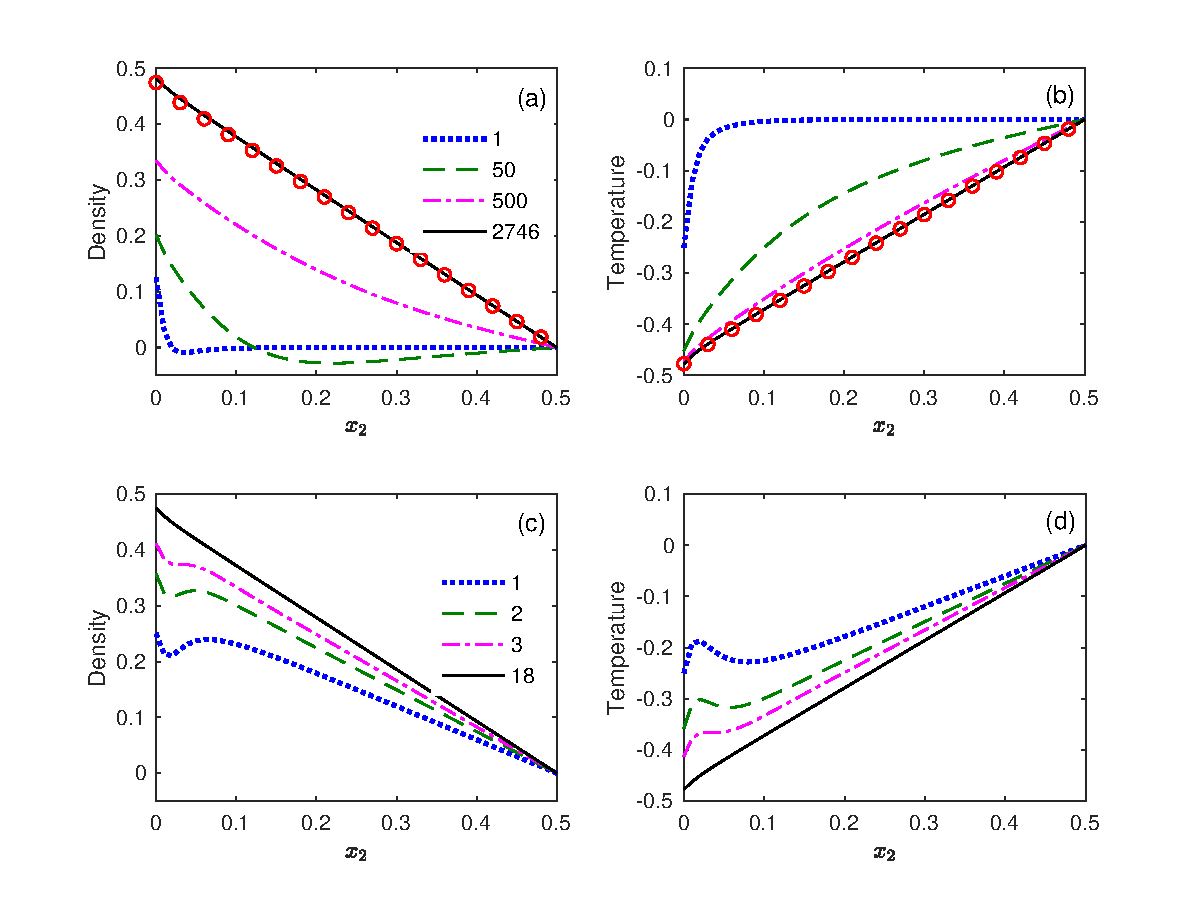
\includegraphics[scale=0.8,viewport=20 10 540 420,clip=true]{Fourier_convergence_history.eps}
	\caption{Density and temperature profiles at different iteration steps obtained from the CIS (a, b) and GSIS (c, d), when the rarefaction parameter is $\delta_{rp} = 50$. Circles show the converged solution obtained from the GSIS. The linearized Shakhov model is used with the initial condition  $h(x_2,\bm{v})=0$. The spatial region is discretized by $N_2=51$ equidistant points. The iteration stops when $\epsilon$ in Eq.~\eqref{epsilon_Fourier} is less than $10^{-5}$. Data in the legends are the iteration steps.}
	\label{fig:Fourier_histroy}
\end{figure}


We first test the efficiency of the GSIS based on the Shakhov model, that is, the linearized Boltzmann collision operator in Eq.~\eqref{Chapter1_Boltzmann_lin} is replaced by the linearized Shakhov model~\eqref{LBE_shakhov}. We choose the rarefaction parameter $\delta_{rp}=50$ and discretize the half spatial space into $N_2$ even-spaced points, where the derivative with respect to $x_2$ is approximated by a second-order upwind finite difference. The molecular velocity space in the $v_1$ and $v_3$ directions is truncated to the region $[-6, 6]$ by $24\times24$ equidistant points, while the molecular velocity $v_2$ is truncated to $[-6,6]$ and approximated by the non-uniform points~\eqref{nonuniform_v},
which is useful to capture the discontinuity in the velocity distribution function near $v_2\sim0$. In this test we take $\imath=3$ and $N_v=64$. The iterations in both CIS and GSIS are terminated when 
\begin{equation}\label{epsilon_Fourier}
\epsilon= \max\left\{
\int{}\left|\frac{\rho^{(k+1)}}{\rho^{(k)}}-1\right|\mathrm{d}x_2, 
\int{}\left|\frac{T^{(k+1)}}{T^{(k)}}-1\right|\mathrm{d}x_2,
\int{}\left|\frac{q_2^{(k+1)}}{q_2^{(k)}}-1\right|\mathrm{d}x_2
\right\}
\end{equation}
is less than a certain value. Note that  $\rho$ and $T$  at $x_2=1/2$ are excluded in the above equation since they are zero.



\begin{figure}[t]
	\centering
	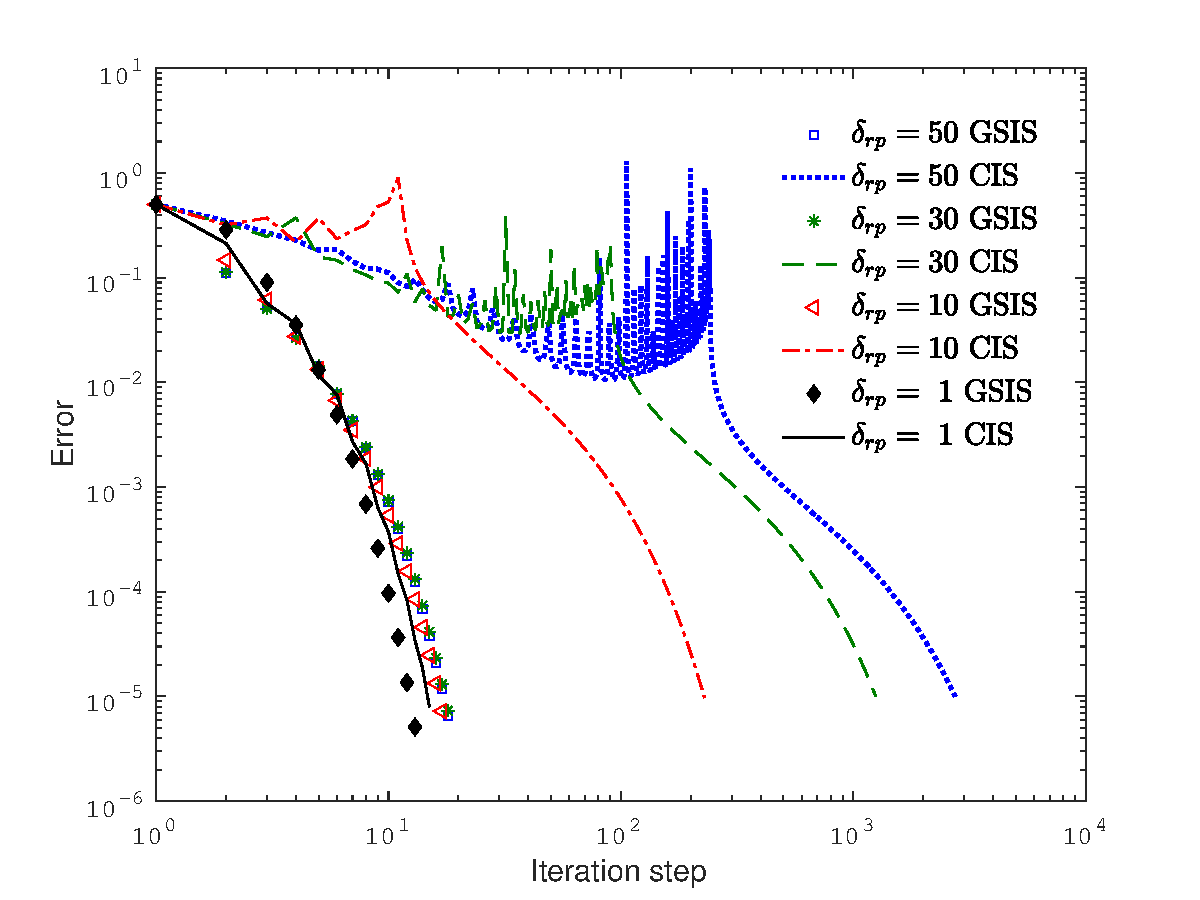
\includegraphics[scale=0.55,viewport=40 20 540 410,clip=true]{Fourier_convergence_error.eps}
	\caption{The decay of the error $\epsilon$ as a function of the iteration step, for the Fourier flow between two parallel plates described by the linearized Shakhov model. The spatial region is discretized by $N_2=51$ equidistant points.  }
	\label{fig:Fourier_speed}
\end{figure}

Figure~\ref{fig:Fourier_histroy} compares the convergence history of the GSIS and CIS when the rarefaction parameter is $\delta_{rp}=50$, that is, the flow is in the near-continuum regime. Starting from the initial guess $h(x_2,\bm{v})=0$, the perturbance from the solid surface quickly changes the density and temperature near the solid surface in the CIS (within about one molecular mean free path away from the wall). However, due to the frequent collision between gas molecules, those in the bulk region takes a long time (i.e. iteration steps) to feel this change. From example, from Fig.~\ref{fig:Fourier_histroy}(b) we see that it takes about 50 iteration steps for the temperature at $x_2=0.5$ to feel this change. Moreover, such a change does not necessary lead to the final converged state monotonically, but it could deviate further away from the final steady state: from Fig.~\ref{fig:Fourier_histroy}(a) we see that the density perturbance in the bulk region is even negative after 50 iterations, while the final steady state the density is always non-negative in the region of $x_2\in[0, 0.5]$. This is also evidenced in Fig.~\ref{fig:Fourier_speed} that the error does not decay monotonically but oscillates several times. Such a slow convergence is completely changed in the GSIS, where the temperature and density are corrected according to the synthetic equations~\eqref{HoT_q_Fourier} and~\eqref{synthetic44}; the dominated parts are respectively $\frac{\partial T}{\partial x_2}=-\frac{4\delta_{rp}}{9C_q}q_{2}$ and $\rho=-T$ when $\delta_{rp}$ is large, and this means that the temperature and density in the bulk region are corrected to be nearly linear immediately. As we can see from Fig.~\ref{fig:Fourier_histroy}(d), after the first iteration, the temperature from the GSIS at $x_2=0$ is the same as that from the CIS, but the temperature from the GSIS in the bulk region varies linearly, while that from the CIS is still zero. From Fig.~\ref{fig:Fourier_histroy}(c) we see that the density also varies linearly in the bulk, but at the solid surface it is more close to the final state than that obtained from the CIS. Since the diffusion-type  macroscopic equation~\eqref{HoT_q_Fourier} allows the efficient exchange of information, fast convergence is realized in the whole computational domain, see Fig.~\ref{fig:Fourier_histroy}(c) and (d).	


%Since the symmetry condition always guarantees $n(x_2=1/2)=T(x_2=1/2)=0$, a large number of iterations are needed to alter the density and temperature profiles between the solid surface and the center of the channel to be nearly linear.


Figure~\ref{fig:Fourier_speed} demonstrates how fast the solution is converged at different values of rarefaction parameter. When $\delta_{rp}$ is small, errors in both the CIS and GSIS decay at the same rate, which means that the two schemes are as efficient as each other. As $\delta_{rp}$ increases so that the flow enters the transition and near-continuum regimes, the error in the CIS oscillates several times before it decays monotonically. As a consequence, the iteration number of CIS increases rapidly with the rarefaction parameter, which nearly scales as $\delta_{rp}^2$. For the GSIS, however, the error is monotonically decreasing, and the rarefaction parameter does not influence the error decay rate, where the converged solutions are obtained within the same number of iterations (here 20 iterations) for each rarefaction parameter from the free molecular to continuum flow regimes. At $\delta=50$, the GSIS is about 100 times more efficient than the CIS, and it can be expected that the gain of using GSIS becomes larger and larger as $\delta_{rp}$ further increases.



\begin{figure}[t]
	\centering
	\includegraphics[scale=0.38,viewport=20 0 540 420,clip=true]{Fourier_density_error.eps}
	\includegraphics[scale=0.38,viewport=20 0 540 420,clip=true]{Fourier_heat_error.eps}
	\caption{The influence of the spatial discretization on the accuracy of both the CIS and GSIS, for the Fourier flow between two parallel plates described by the linearized Shakhov model with $\delta_{rp}=50$. The iteration terminates when $\epsilon<10^{-6}$. The reference solutions (i.e. $\rho_{ref}$ and $q_{2,ref}$) are obtained from the GSIS with $N_2=251$, that is, the spatial cell size is about one tenth of the mean free path of gas molecules.}
	\label{fig:Fourier_spatial_error}
\end{figure}


Another important property of the GSIS is that the numerical error caused by the spatial discretization is much reduced when compared to that of the CIS.  From Fig.~\ref{fig:Fourier_spatial_error} we see that when $N_2$ is decreased from 251 to 6, that is, when the spatial cell size is respectively about $1/10$ and 5 times of the mean free path of gas molecules, the relative error in the density profile increases from 0.3\% to 9\%, while that in the heat flux increases from 0.3\% to 16\% in the CIS. However, the relative error in the GSIS always remain within 1\%, even when the cell size is about 5 times larger than the gas mean free path. Note that even when $\delta_{rp}=500$, the heat flux obtained from the GSIS only changes from $3.721\times10^{-3}$ when $N_2=551$ to $3.726\times10^{-3}$ when $N_2=6$. The reason for this excellent performance is that the GSIS is asymptotically preserving the Navier-Stokes limit, while in the CIS the ``numerical'' thermal conductivity may be different to the physical one. Besides, in the CIS, the false convergence, e.g. the non-uniform distribution of heat flux in Fig.~\ref{fig:Fourier_spatial_error}(b), may be reached when the spatial resolution is not enough. The superior GSIS,  however, does not suffer this problem.


It should be noted that the implicit UGKS~\cite{Zhu2019JCP} and other variants~\cite{yang2018PoF,yang2018PRE} can also produce accurate results when the cell size is much larger than the molecular mean free path. This is achieved through a complex evaluation of the numerical flux at the cell interface to spontaneously treat the molecular streaming and collision. The GSIS, however, does not need complex flux evaluation since the Navier-Stokes constitutive laws are recovered explicitly. 



Using the accurate and efficient GSIS, the LBE is solved for different molecular collision models~\eqref{collision_kernel} and the corresponding Knudsen layer functions are obtained. In the numerical simulation, we set the rarefaction parameter to be $\delta_{rp}=60$, so that the distance between two plates is about 60 times as large as the mean free path of gas molecules; thus, the interference between the Knudsen layers near each plate is avoided. In the fast spectral approximation of the linearized Boltzmann collision operator~\eqref{LBE_collision}, the integral with respect to the solid angle $\Omega$ is calculated by the Gauss-Legendre quadrature with $M=6$, see Eq.~(39) in Ref.~\cite{Lei2013}. In the spatial discretization we let
\begin{equation}\label{space_discrete}
x_2=(10-15s+6s^2)s^3, \quad s=(0,1,\cdots,N_s-1)/2(N_s-1)
\end{equation}
with $N_s=200$. The iteration is terminated when $\epsilon<10^{-6}$.




\lei{When the LBE for HS, Helium and Maxwell molecules is solved by the GSIS, steady-state solutions are reached after 22, 25 and 27 iterations, respectively, and the temperature jump coefficients are respectively 1.892,1.933 and 1.954, which do not differ a lot between the three collision models.} However, the Knudsen layer functions shown in Fig.~\ref{fig:Fourier_Knudsen_layer} have larger difference. It is amazing that the small terms $2\int{(L-L_s)v_iv_j}\mathrm{d}\bm{v}$ in Eq.~\eqref{HoT_sigma} and $\int{(L-L_s)v_iv^2} \mathrm{d}\bm{v}$ in Eq.~\eqref{HoT_q} significantly affect the Knudsen layer function.

When the macroscopic flow variables are solved by SIMPLE algorithm, the velocity distribution function is updated as
\begin{equation}
\begin{aligned}[b]
h^{(k+1)}(\bm{x},\bm{v})=&h^{(k+1/2)}(\bm{x},\bm{v})\\
&+\frac{\delta_{rp}}{\max(10,\delta_{rp})}\left[\lambda_{\rho}(\bm{x})
+2\lambda_{\bm{u}}(\bm{x})\cdot{\bm{v}}
+\lambda_T(\bm{x})\left(v^2-\frac{3}{2}\right)
\right]f_{eq},
\end{aligned}
\end{equation}
because (i) the update of the shear stress and heat flux does not affect the accuracy and efficiency of the GSIS, and (ii) for highly rarefied gas flows, high-order terms are very large and the macroscopic synthetic equations become stiff near the solid corners due to the small value of $\delta_{rp}$, hence the limiter ${\delta_{rp}}/{\max(10,\delta_{rp})}$ is introduced to increase the numerical stability.




%We first test the converging speeds of both CIS and GSIS for the cases of $\delta_{rp} = 0.1$, 1, 10, 100 and 1000. The corresponding spatial grids are non-uniform with $N_s=21$, 21, 21, 41, 61 respectively. For the cases of $\delta_{rp} = 0.1$, 1 and 10, the molecular velocity in both $v_1$ and $v_2$ are discretized by Eq.~\eqref{nonuniform_v}, with $\imath=3$, and $N_v=48$, 48 and 24, respectively, while for $v_3$, 24, 24 and 12 uniform points in the range of $[-6,6]$ are used, respectively. When $\delta=100$ and 1000, the 6- and 8-point Gauss-Hermite quadrature nodes are used in all three velocity components. The iterations in both CIS and GSIS are assumed to be converged when
%\begin{equation}\label{error_lid}
%\epsilon=\iint \left | \frac{|\bm U^{(k+1)}|}{|\bm U^{(k)}|} - 1 \right |\mathrm{d}x_1\mathrm{d}x_2 < 10^{-5}.
%\end{equation}


\subsection{Couette flow between two eccentric cylinders}



In this section, we consider a Couette flow between two noncoaxial cylinders. This test case is used to show that the proposed GSIS can be efficiently implemented through other CFD method rather than the finite difference algorithm to deal with more complicated geometries. As shown in Fig.~\ref{CylinderG}, the outer cylinder with a radius of 2 rotates clockwise at a constant speed of $U_w$, while the inner cylinder with a radius of 1 keeps static. The centers of the outer cylinder and inner cylinder are at $\bm{x}=(0,0.5)$ and the origin, respectively. Both cylinders have a constant temperature $T_0$. It is assumed that $U_w$ is much smaller than the most probable speed $v_m$, thus the gas system can be linearized with $\alpha=U_w/v_m$. The velocity distribution function for  reflected molecules at the outer cylinder is given by

\begin{equation}
\begin{aligned}
h\left(\bm{x},\bm{v}\right)=\left[2\bm{t}_w\cdot\bm{v}-2\sqrt{\pi}\int_{\bm{v}'\cdot\bm{n}_w<0}\bm{v}'\cdot\bm{n}_wh\left(\bm{x},\bm{v}'\right)\mathrm{d}\bm{v}'\right]f_{eq},
\end{aligned}
\end{equation}
when $\bm{v}\cdot\bm{n}_w>0$,
where $\bm{n}_w$ and $\bm{t}_w$ denote the outward unit normal vector and tangential vector of the solid surface. The boundary condition at the inner cylinder is similar but without the term $\bm{t}_w\cdot\bm{v}$.



%\begin{figure}[t]
%	\begin{center}
%		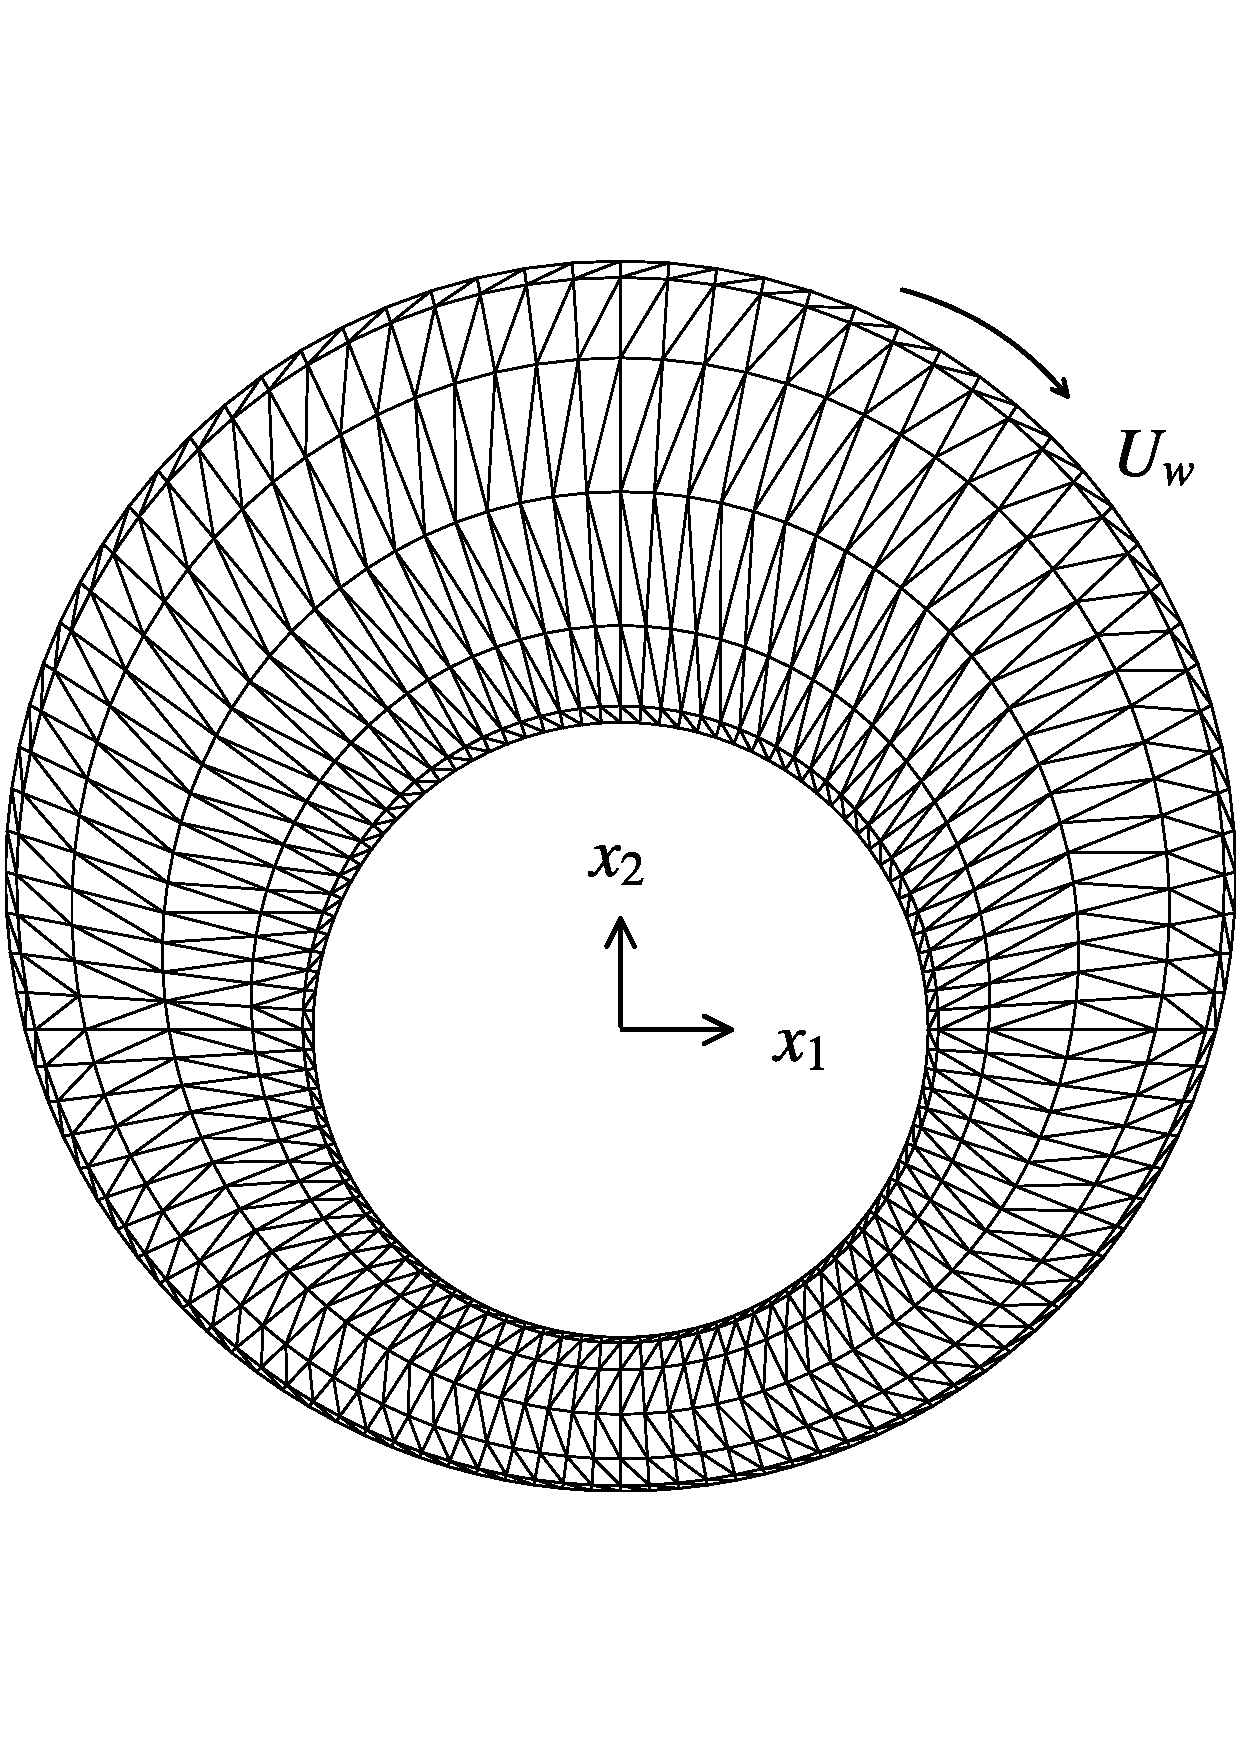
\includegraphics[width=0.3\textwidth]{Cylinder_G.pdf}
%	\end{center}
%	\caption{Schematic of the geometry and structured triangular mesh for shear-driven flow between two eccentric cylinders.}
%	\label{CylinderG}
%\end{figure}

\begin{figure}[p]
	\centering
	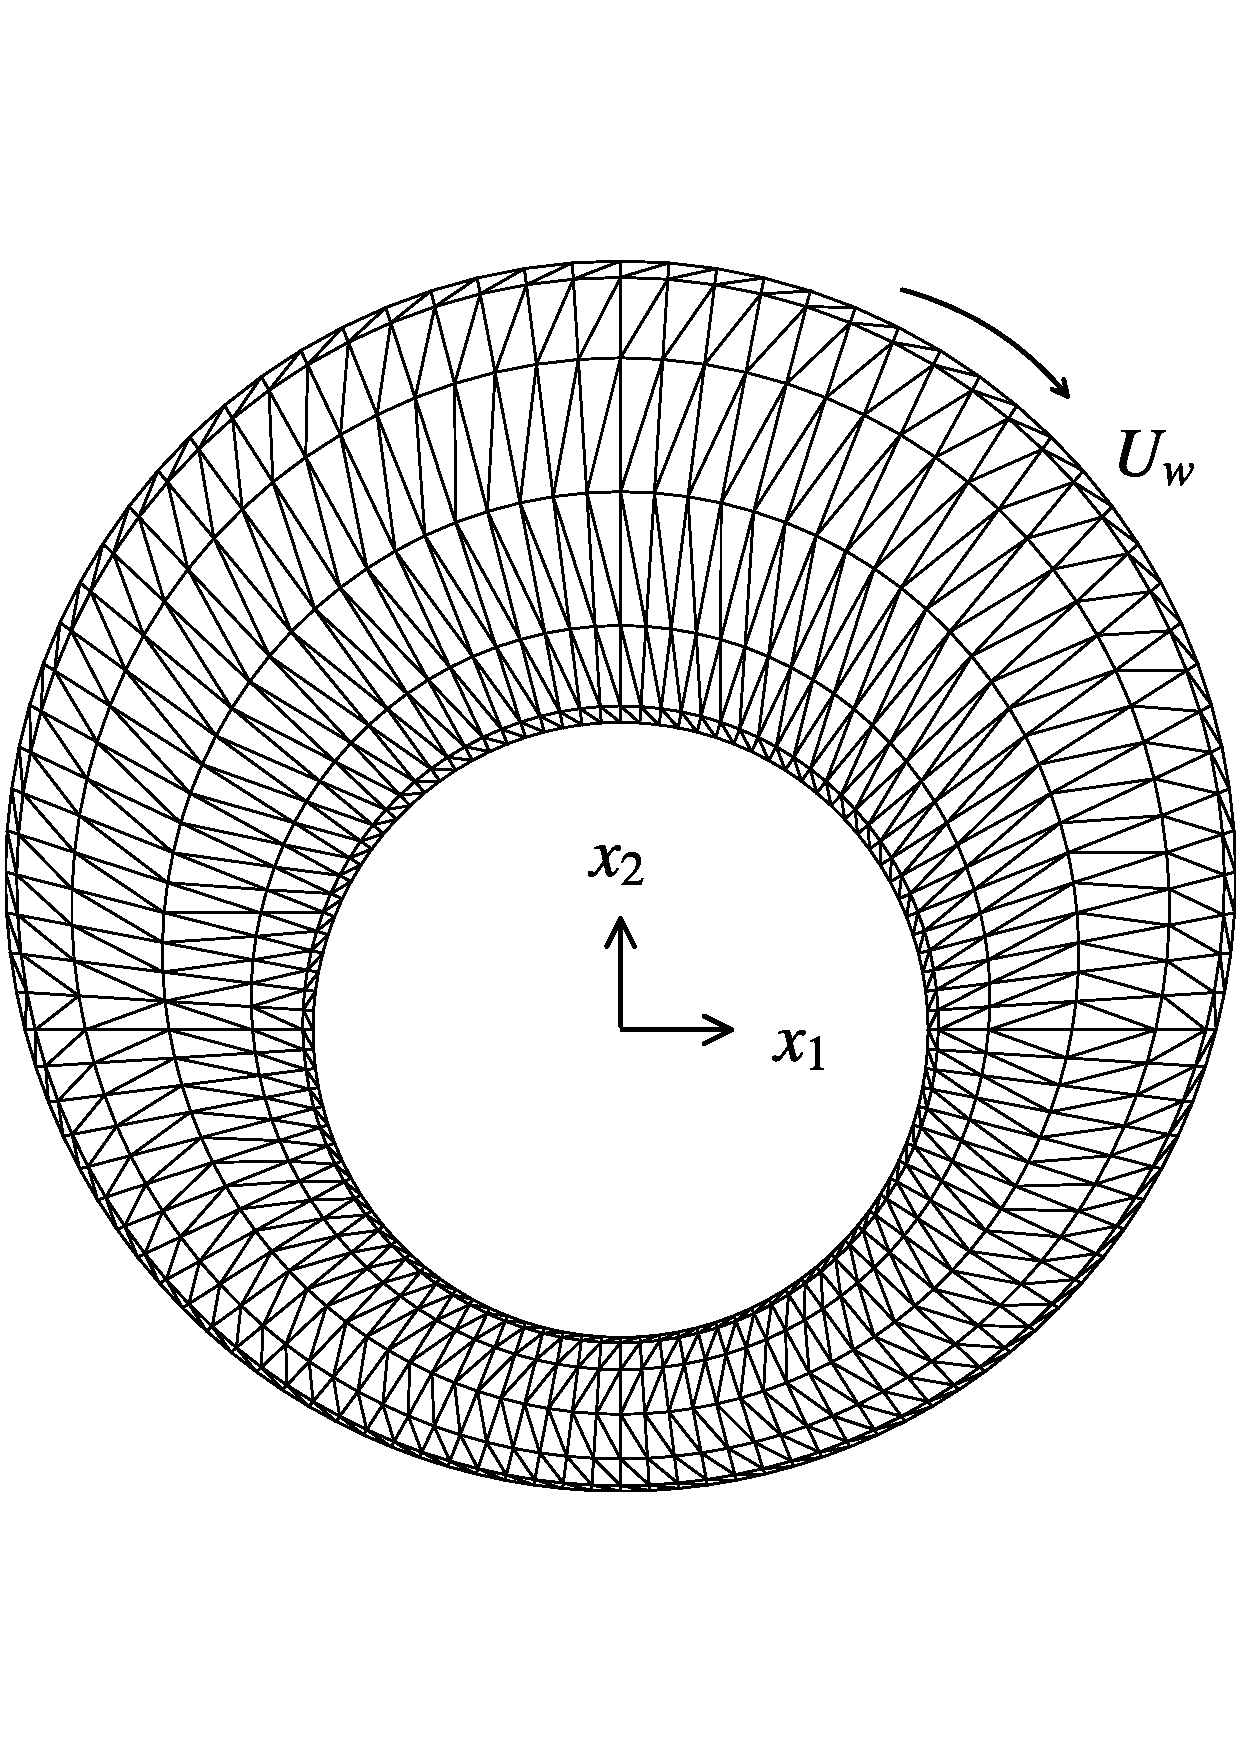
\includegraphics[width=0.3\textwidth]{Cylinder_G.pdf}\\
	\vskip 0.5cm
	\includegraphics[width=0.4\textwidth]{TwoCylinderD1000u.pdf}\hskip 0.5cm
	\includegraphics[width=0.4\textwidth]{TwoCylinderD1000v.pdf}
	\vskip 0.5cm
	\includegraphics[width=0.4\textwidth]{TwoCylinderD10u.pdf}\hskip 0.5cm
	\includegraphics[width=0.4\textwidth]{TwoCylinderD10v.pdf}
	\caption{Comparisons of the CIS and GSIS results for shear-driven flow between two eccentric cylinders. (a) Contours of $U_1$ and streamlines at $\delta_{rp}=1000$; (b) Contours of $U_2$ and streamlines at $\delta_{rp}=1000$; (c) Contours of $U_1$ and streamlines at $\delta_{rp}=10$; (d) Contours of $U_2$ and streamlines at $\delta_{rp}=10$. In each sub-figures, the GSIS results are plotted in the left half domain while the CIS ones are illustrated in the right half domain. In (a) and (b) the velocity contours obtained by only solving the Navier-Stokes equations with non-slip velocity boundary are also included, which are indicated by the white dashed lines.
	}
	\label{TwoCylinderV}
\end{figure}

Using both the GSIS and CIS, the shear-driven flow is simulated on structured triangular mesh, in which the grid nodes along the radial direction is described by Eq.~\eqref{Couette_spatial_grid}. The high-order DG methods are employed to seek solutions of the linearized Shakhov model equation and the synthetic macroscopic equations, in pecewise polynomial spaces of degree of 3. The detailed DG scheme for the gas kinetic equation can be found in~\cite{Su2019IDG}, while the hybridizable DG algorithm to solve the synthetic macroscopic equations is listed in the Appendix. 




The resultant velocity contours and streamlines are illustrated in Fig.~\ref{TwoCylinderV} for two selected rarefaction parameters $\delta_{rp}=1000$ and 10, in which the GSIS solutions are plotted in the left half domain and the CIS ones are plotted in the right half domain. The results at $\delta_{rp}=1000$ are obtained on 2400 triangles with cell size (characterized by the height of triangle) varying from 3 to 260 times the mean free path of gas molecules. The molecule velocity space is discretized by 8-point Gauss-Hermite quadrature nodes in $v_1$ and $v_2$ and 12 equidistant nodes in the range of $[-4,4]$ in $v_3$. The results at $\delta_{rp}=10$ are obtained on 1600 triangles with cell size varying from 0.1 to 3 times the mean free path of gas molecules. The molecule velocity space is discretized in the domain of $[-4,4]^3$ by 32 non-uniform nodes in $v_1$ and $v_2$ and 24 equidistant nodes in $v_3$. Numerical solutions are believed to be converged when the relative error in velocity magnitude $|\bm{u}|$ between two consecutive iteration steps is less than $10^{-5}$. The streamlines show that, as the gas rotates clockwise from the top to the bottom, due to the shrink of the flow pass, part of the gas near the outer surface is squeezed into the bottom narrow space while the other part of the gas flows back along the surface of the inner cylinder; as a consequence, a vortex appears above the inner cylinder. 


Large discrepancies in the velocity contours are observed between the GSIS and CIS results at $\delta_{rp}=1000$. To test the accuracy of both schemes, we also include the results of the Navier-Stokes equations with the non-slip velocity boundary condition, which are illustrated by the white dashed lines in Fig.~\ref{TwoCylinderV}(a) and (b). The GSIS results overlap with the ones from the Navier-Stokes equations, thus the GSIS can asymptotically preserve the Navier-Stokes limit. However, the CIS cannot predict accurate solutions due to the large numerical dissipation on such a coarse mesh, i.e. the maximum cell size is about 260 times of the molecular mean free path.  As the rarefaction parameter decreases to 10, the GSIS and CIS can produce close solutions on the same mesh. 

Consider the rate of convergence to the steady-state solution, the numbers of iteration steps and CPU time to reach convergence for both the CIS and GSIS are listed in Table~\ref{tab:iteration2}. All the cases are done in double precision on Intel Xeon-E5-2680 processors and 128 GB RAM and the direct sparse solver, PARDISO~\cite{pardiso} is called to directly solve the linear system for macroscopic equations. The simulations are run on 12 processors using OpenMP. It is seen that the GSIS cost only 26 iterative steps to reach the convergence criterion for both the cases of $\delta_\text{rp}=1000$ and 10, while the CIS consumes 49454 and 296 steps, respectively. Compared to that of solving the kinetic equation, the computational consumption for DG to solve the macroscopic equations is very little, since the number of degrees of freedom for the latter one is much smaller. Therefore, the GSIS can be nearly 1300 and 5 times faster than the CIS when $\delta_\text{rp}=1000$ and 10, respectively.


\begin{table}[t]
	\centering
	\caption{Number of iteration steps and CPU time to reach convergence for the shear-driven flow between two eccentric cylinders. }
	\begin{tabular}{rllrrrr}
		\hline
		\multicolumn{1}{l}{$\delta_\text{rp}$} & \# of triangles & $N_{v_1}N_{v_2}N_{v_3}$    & \multicolumn{2}{c}{Iteration steps} & \multicolumn{2}{c}{Total CPU time (s)} \\ 
		&       &       & \multicolumn{1}{r}{CIS} & \multicolumn{1}{r}{GSIS} & \multicolumn{1}{r}{CIS} & \multicolumn{1}{r}{GSIS}\\ 
		\hline
		1000   & 2400 & $8\times8\times 12$ & 49454    & 26    &     33861.2  & 26.3 \\
		10  & 1600 & $32\times32\times 24 $& 296    & 26    &   2849.8    & 580.3 \\ 
		\hline
	\end{tabular}%
	\label{tab:iteration2}%
\end{table}














\section{Molecular gas}

Wei's CMAME paper
\newpage
a
\newpage
b
\newpage


\section{Time-dependent and nonlinear problems}

Scheme II

\newpage
a
\newpage
b
\newpage


\section{Conclusions and outlooks}\label{sec:summary}


In summary, we have developed a general synthetic iterative scheme to find the steady-state solution of the linearized Boltzmann equation efficiently and accurately. Various numerical results have demonstrated that our scheme is able to find the converged solution within about 20 iterations at any Knudsen number, due to the fact that the synthetic macroscopic equations not only asymptotically preserves the Navier-Stokes limit in the framework of Chapman-Enskog expansion, but also explicitly contain the constitutive laws for the stress and heat flux at the first order approximation in the the Knudsen number to the linearized Boltzmann equation. As a consequence, accurate solutions that are not contaminated by numerical dissipation and accumulated error can be obtained when the cell size is much larger than the mean free path of gas molecules. Moreover, the numerical error in the general synthetic iterative scheme decays very fast and the convergence criterion can be set at a much higher value than the conventional iterative scheme. These factors enables our general synthetic iterative scheme to find the steady-state solution in 10-ish iterations.

\leir{Some one may criticize that macroscopic equations pulls the solution directly to NS, this is actually not, as when Kn is very small, the Knudsen layer is recovered and usually different molecular model lead to different values of KLF, see Chapter~\ref{chap:velocity_slip} below }

This paper provides a framework to solve the general linear rarefied gas flow problems. \leir{The essence of our approach relies on the following two points: (i) the explicit inclusion of Navier-Stokes constitutive laws and (ii) high-order terms are derived exactly from the gas kinetic equation. The first point ensures fast convergence in the (near) continuum flow regime, while the latter ensures that correct solution is obtained in transition and free-molecular flow regimes.} The advantages and future works are highlighted below:
\begin{enumerate}
	
	\item Compared to the implicit UGKS~\cite{Zhu2019JCP} and it variants~\cite{yang2018PoF,yang2018PRE}, we conclude that in order to develop efficient multiscale numerical schemes, macroscopic equations must be solved together with the Boltzmann or kinetic model equations. While in Refs.~\cite{Zhu2019JCP,yang2018PoF,yang2018PRE} only five equations from the conservation laws are used so that complex flux evaluation across the cell interface must be adopted to asymptotically preserve the Navier-Stokes limit, our general synthetic iterative scheme needs no flux evaluation as the Navier-Stokes equations are recovered explicitly. Thus, the numerical implementation of GSIS is much easy than UGKS and the convergence to steady-state solution is much faster. More importantly, our scheme does not depend on the specific form of the collision operator, while that in Refs.~\cite{Zhu2019JCP,yang2018PoF,yang2018PRE} relies only on the BGK-type kinetic equations to enable exact evaluation of numerical flux. 
	
	\item \leir{The gas kinetic equation and synthetic equations can be solved by sophisticated methods in computational fluid dynamics. For highly rarefied gas flows, the cell size is usually smaller than the mean free path and both methods yield high accuracy. For continuum/or near continuum flows, as long as the macroscopic solver for synthetic equations (essentially the NS equations) is able to capture the continuum flow behaviors, the accuracy of GSIS is guaranteed, that is, the numerical cell size can be much larger than the MFP, but should be smaller than the variation scale (such as the wavelength of sound) of the flow. In other words, the solution of GSIS is not affected when gas kinetic equation and synthetic equations are discretized by different schemes, as long as synthetic equation captures the flow dynamics in the continuum regime. For example, in Fourier/oscillating Couette/sound propagation problems, the gas kinetic equation is solved by the second-order upwind finite difference, while synthetic equations are solved by central finite difference.  } 
	
	\item Since the limitation on spatial cell size (i.e. it should be smaller than the mean free path of gas molecules) is removed and fast convergence is enabled, the present general synthetic iterative scheme may be applied to low-variance~\cite{Radtke2009PRE,Radtke2011} and even frequency-domain~\cite{Ladiges2015JCP} DSMC that solves the linearized Boltzmann and kinetic model equations to improve the computational efficiency, especially in the near-continuum flow regime. 
	
	
	\item The present method can be extended to multi-species and compressible flow. The key is to construct macroscopic equations that recover the compressible Navier-Stokes equation to the first order of Knudsen number. As a matter of fact, the Grad 13 moment equations~\cite{Grad1949,henning} can be directly used if the high-order velocity moments are calculated from the numerical solution of the Boltzmann equation, rather than closed by making assumption on the form of velocity distribution function. 
	
	\item 
We believe that the general synthetic iterative scheme can also be applied to DSMC to remove the limitation on cell size and boost convergence, and the advantage is clear: it relies on no specific collision operator so that can be extended naturally to multi-species flows and even flows involving chemical reactions.
	
\end{enumerate}  


With these new development implemented, it is foreseen that in the near future the problem of numerical simulation of multiscale rarefied gas flows may be solved completely. Also, the same idea can be applied to other kinetic equations such as the Enskog equation for dense gases dynamics with applications to gas extraction in unconventional reservoirs and non-equilibrium evaporation and condensation at the nano scale~\cite{Lei2015Enskog,Wu2016JFM,Frezzotti2005}.






%\appendix
%
%\section*{Appendix}
%\renewcommand{\theequation}{A.\arabic{equation}}
%
%Here, some details to solve the synthetic macroscopic equations using the high-order hybridizable discontinuous Galerkin (HDG) method~\cite{Cockburn2010} on arbitrary triangular mesh are presented. The steady-state governing equations can be written in the following mixed form as a system of first-order equations
%\begin{equation}
%\begin{aligned}[b]
%\nabla\cdot\left[\bm{\mathcal{G}}_\text{c}+\bm{\mathcal{G}}_\text{d}\right]=0,\\
%\bm{L}-\nabla\bm u-\bm{\Pi}=0,\\
%\bm{E}-\nabla T-\bm{\Theta}=0,
%\end{aligned}
%\end{equation}
%where
%\begin{equation}
%\begin{aligned}[b]
%\bm{\mathcal{G}_\text{c}}=\left[\begin{array}{c}
%\bm U\\p\bm I\\\bm 0
%\end{array}
%\right],\\
%\bm{\mathcal{G}_\text{d}}=\left[\begin{array}{c}
%\bm 0\\-\frac{1}{\delta_{rp}}\left(\bm L+\bm L^{\text{T}}-\frac{2}{3}\mathrm{tr}\left(\bm L\right)\bm I\right)\\
%-\frac{5}{4\delta_{rp}\mathrm{Pr}}\bm E
%\end{array}
%\right],\\
%\bm{\Pi}=\left[\begin{array}{cc}
%\text{HoT}_{\sigma_{11}}+\frac{1}{2}\text{HoT}_{\sigma_{22}} & \frac{1}{2}\text{HoT}_{\sigma_{12}}\\
%\frac{1}{2}\text{HoT}_{\sigma_{12}} & \frac{1}{2}\text{HoT}_{\sigma_{11}}+\text{HoT}_{\sigma_{22}}
%\end{array}
%\right],\\
%\bm{\Theta}=\left[\begin{array}{c}
%\frac{4}{5}\text{HoT}_{q_{1}} \\
%\frac{4}{5}\text{HoT}_{q_{2}} 
%\end{array}
%\right],
%\end{aligned}
%\end{equation}
%with $\bm{I}$ being the identity matrix. The auxiliary variables $\bm{L}$ and $\bm{E}$ are introduced to approximate the combination of the velocity gradient $\nabla\bm{u}$, temperature gradient $\nabla T$ and the high-order moments. Then, the stress tensor and heat flux are evaluated as
%\begin{equation}\label{sq}
%\sigma_{ij}=-\frac{1}{\delta_{rp}}\left(L_{ij}+L_{ji}-\frac{2}{3}L_{kk}\delta_{ij}\right),\quad q_i=-\frac{5}{4\delta_{rp}\mathrm{Pr}}E_i.
%\end{equation}
%
%Let $\Delta\in\mathbb{R}^2$ be an two-dimensional domain with boundary $\partial\Delta$ in the $x_1-x_2$ plane. Then, $\Delta$ is partitioned in $M$ disjoint regular triangles $\Delta_i$: $\Delta=\cup^{M}_i\Delta_i$. The boundaries $\partial\Delta_i$ of the triangles define a group of $N$ faces $\Gamma_c$: $\Gamma=\cup^{M}_i\{\partial\Delta_i\}=\cup^{N}_c\{\Gamma_c\}$. For HDG discretization, two types of discontinuous finite element approximation space, one for solutions within $\Delta_i$ and the other for traces of solution on $\Gamma_c$, are defined as
%\begin{equation}
%\begin{aligned}[b]
%\mathcal{V}=\{\varphi:\ \varphi|_{\Delta_i}\in\mathcal{P}^k(\Delta_i),\ \forall\ \Delta_i\subset\Delta\},\\
%\mathcal{W}=\{\psi:\ \psi|_{\Gamma_c}\in\mathcal{P}^k(\Gamma_c),\ \forall\ \Gamma_c\subset\Gamma\},
%\end{aligned}
%\end{equation}
%where $\mathcal{P}^k(D)$ denotes the space of $k-$th order polynomials on a domain $D$. 
%
%
%The HDG method solves the system in two steps. First, a global problem is set up to determine the traces of the flow properties $\hat{\bm{Q}}=\left[\hat{p},\hat{\bm{u}},\hat{T}\right]$ on the faces $\Gamma$. Then, a local problem with $\hat{\bm{Q}}$ as the boundary condition on $\partial\Delta_i$ is solved element-by-element to obtain the solutions for the flow properties $\bm{Q}=\left[p,\bm{Q},T\right]$, as well as the ones for the auxiliary variables $\bm{L}$ and $\bm{E}$. Generally speaking, when moving from the interior of the triangle element $\Delta_i$ to its boundary $\partial\Delta_i$, the traces defines what the values of field variables on the boundary should be. In the HDG method, it is assumed that the traces are singled-valued on each face. 
%
%We introduce the notations $\left(a,b\right)_D=\int_{D\in\mathbb{R}^2}\left(a\odot b\right)\mathrm{d}x_1\mathrm{d}x_2$ and $\langle a,b\rangle_D=\int_{D\in\mathbb{R}^1}\left(a\odot b\right)\mathrm{d}\Gamma$, where $\odot$ can be either the dot product $\cdot$ or tensor product $\otimes$. The local problem is stated as: find $\left(\bm{Q},\bm{L},\bm{E}\right)\in\left[\mathcal{V}\right]^4\times\left[\mathcal{V}\right]^4\times\left[\mathcal{V}\right]^2$ such that
%\begin{equation}\label{local}
%\begin{aligned}[b]
%-\left(\bm{\mathcal{G}_\text{c}}+\bm{\mathcal{G}_\text{d}},\nabla\bm{r}\right)_{\Delta_i}+\langle\hat{\bm{\mathcal{F}}}\cdot\bm{n},\bm{r}\rangle_{\partial\Delta_i}=0,\\
%\left(\bm{L},\bm{w}\right)_{\Delta_i}+\left(\bm{u},\nabla\cdot\bm{w}\right)_{\Delta_i}-\langle\hat{\bm{u}},\bm{w}\cdot\bm{n}\rangle_{\partial\Delta_i}=\left(\bm{w},\bm{\Pi}\right)_{\Delta_i},\\
%\left(\bm{E},\bm{z}\right)_{\Delta_i}+\left(T,\nabla\cdot\bm{z}\right)_{\Delta_i}-\langle\hat{T},\bm{z}\cdot\bm{n}\rangle_{\partial\Delta_i}=\left(\bm{z},\bm{\Theta}\right)_{\Delta_i},
%\end{aligned}
%\end{equation}  
%for all $\left(\bm{r},\bm{w},\bm{z}\right)\in\left[\mathcal{V}\right]^4\times\left[\mathcal{V}\right]^4\times\left[\mathcal{V}\right]^2$. The numerical flux $\hat{\bm{\mathcal{F}}}\cdot\bm{n}$ is defined as~\cite{Peraire2010}
%\begin{equation}
%\hat{\bm{\mathcal{F}}}\cdot\bm{n}=\left[\begin{array}{c}
%\bm{u}\\
%\hat{p}\bm{I}-\frac{1}{\delta_{rp}}\left(\bm{L}+\bm{L}^{\mathrm{T}}-\frac{2}{3}\mathrm{tr}\left(\bm L\right)\bm{I}\right)\\
%-\frac{5}{4\delta_{rp}\mathrm{Pr}}\bm{E}
%\end{array}\right]\cdot\bm{n}+\left[\begin{array}{ccc}
%\tau & &\\
%& \frac{\tau}{\delta_{rp}} &\\
%& & \frac{5\tau}{4\delta_{rp}\mathrm{Pr}}
%\end{array}
%\right]\left[\begin{array}{c}
%p-\hat{p}\\
%\bm{u}-\hat{\bm U}\\
%T-\hat{T}
%\end{array}\right].
%\end{equation}
%Here $\bm{n}$ being the outward unite normal vector of $\partial\Delta_i$. $\tau$ is the stabilization parameter that have important effects on the accuracy and convergence of the HDG method. In this work, we chosen $\tau=1/H_\text{min}$, with $H_\text{min}$ the minimum height of the triangles $\Delta_i$. 
%
%The global problem is set up by enforcing the continuity of the numerical flux over all the interior faces. It is stated as: find $\hat{\bm{Q}}\in\left[\mathcal{W}\right]^4$ such that
%\begin{equation}\label{Global1}
%\langle\bm{\left(\hat{\mathcal{F}}}\cdot\bm{n}\right)^+,\bm{\psi}\rangle_{\Gamma_c}+\langle\bm{\left(\hat{\mathcal{F}}}\cdot\bm{n}\right)^-,\bm{\psi}\rangle_{\Gamma_c}=0,\quad\text{on}\ \Gamma_c\in\Gamma\backslash\partial\Delta,
%\end{equation}
%for all $\bm{\psi}\in\left[\mathcal{W}\right]^4$. Here the superscripts $\pm$ denote the numerical fluxes obtained from the triangles on both sides of the face. Note that the traces on boundary faces are calculated as
%\begin{equation}\label{Global2}
%\langle\hat{\bm Q}-\bm{Q}^+_{VDF},\bm{\psi}\rangle_{\Gamma_c},\quad\text{on}\ \Gamma_c\in\Gamma\cap\partial\Delta,
%\end{equation}
%where $\bm{Q}^+_{VDF}$ is the field solutions directly calculated from the approximated velocity distribution function (see Eq.~\eqref{MP}) within the triangle where the boundary face $\Gamma_c$ belongs to. 
%
%By assembling the local problem~\eqref{local} and global problem~\eqref{Global1} and~\eqref{Global2} over all the triangles and faces, we can obtain a matrix system of form
%\begin{equation}
%\left[\begin{array}{cccc}
%A_Q & A_L & A_E & A_{\hat{Q}}\\
%B_Q & B_L & B_E & B_{\hat{Q}}\\
%C_Q & C_L & C_E & C_{\hat{Q}}\\
%D_Q & D_L & D_E & D_{\hat{Q}}\\
%\end{array}
%\right]\left[\begin{array}{c}
%\mathbb{Q}\\
%\mathbb{L}\\
%\mathbb{E}\\
%\hat{\mathbb{Q}}
%\end{array}
%\right]=\left[\begin{array}{c}
%S_{Q}\\
%S_{L}\\
%S_{E}\\
%S_{\hat{Q}}
%\end{array}
%\right],
%\end{equation}
%where $\mathbb{Q}$, $\mathbb{L}$, $\mathbb{E}$ and $\hat{\mathbb{Q}}$ are the vectors of degrees of freedom of the flow properties $\bm{Q}$, the auxiliary variables $\bm{L}$ and $\bm{E}$, and the trace of the flow properties $\hat{\bm{Q}}$, respectively. Note that the degrees of freedom for $\bm{Q}$, $\bm{L}$ and $\bm{E}$ are grouped together and ordered element-by-element, and the corresponding coefficient matrix $\left[A_Q,A_L,A_E;B_Q,B_L,B_E;C_Q,C_L,C_E\right]$ has block-diagonal structure. Therefore, we can eliminate $\bm{Q}$, $\bm{L}$ and $\bm{E}$ to obtained a reduced linear system involving only $\hat{\mathbb{Q}}$. Once $\hat{\mathbb{Q}}$ is determined, $\bm{Q}$, $\bm{L}$ and $\bm{E}$ are reconstructed corresponding to the local problem~\eqref{local} in an element-wise fashion, while the stress tensor and heat flux are calculated as Eq.~\eqref{sq}.

    


